% Seminar 2: ARMA models
% Time Series Analysis -- Bachelor's programmes Economic Informatics and Economic Cybernetics, Bucharest University of Economic Studies
% GENERATED by latex/build_seminar2.py -- edit the generator, not this file.
% Student version by default; the instructor version is the *_solutions.tex wrapper.
\makeatletter\@ifundefined{ifsolutions}{\expandafter\newif\csname ifsolutions\endcsname}{}\makeatother

\newcommand{\coursename}{Time Series Analysis}
% Preambul comun TSA -- Serii de timp / Time Series Analysis (Beamer, 16:9)
% Același design ca MFM și SFM (preluat din SFM, 5 octombrie 2026). Înainte de % Preambul comun TSA -- Serii de timp / Time Series Analysis (Beamer, 16:9)
% Același design ca MFM și SFM (preluat din SFM, 5 octombrie 2026). Înainte de % Preambul comun TSA -- Serii de timp / Time Series Analysis (Beamer, 16:9)
% Același design ca MFM și SFM (preluat din SFM, 5 octombrie 2026). Înainte de \input{../../latex/preamble} se definește
%   \newcommand{\coursename}{Time Series Analysis}      (EN)
%   \newcommand{\coursename}{Serii de timp}       (RO)  și  \def\tsalang{ro}
% Fișierele .tex se află în EN/Courses, EN/Seminars, RO/Cursuri, RO/Seminarii (două niveluri sub rădăcină).
% Deck-urile sînt generate de latex/build_chapterN.py / build_seminarN.py (vezi latex/tsa_build.py).

\documentclass[9pt, aspectratio=169, t]{beamer}
\providecommand{\coursename}{Time Series Analysis}

% Ensure content fits on slides
\setbeamersize{text margin left=8mm, text margin right=8mm}
% Smaller institute font (title page)
\setbeamerfont{institute}{size=\footnotesize}

%=============================================================================
% THEME AND STYLE CONFIGURATION
%=============================================================================
\usetheme{default}
% Using default theme for clean header/footer control

% Color Palette (matching Redispatch PDF)
\definecolor{MainBlue}{RGB}{26, 58, 110}
\definecolor{AccentBlue}{RGB}{26, 58, 110}
\definecolor{IDAred}{RGB}{205, 0, 0}
\definecolor{DarkGray}{RGB}{51, 51, 51}
\definecolor{MediumGray}{RGB}{128, 128, 128}
\definecolor{LightGray}{RGB}{248, 248, 248}
\definecolor{VeryLightGray}{RGB}{235, 235, 235}
\definecolor{KeynoteGray}{RGB}{218, 218, 218}
\definecolor{SectionGray}{RGB}{120, 120, 120}
\definecolor{FooterGray}{RGB}{100, 100, 100}
\definecolor{Crimson}{RGB}{220, 53, 69}
\definecolor{Forest}{RGB}{46, 125, 50}
\definecolor{Amber}{RGB}{181, 133, 63}
\definecolor{Orange}{RGB}{230, 126, 34}
\definecolor{Purple}{RGB}{142, 68, 173}

% Gradient background (exact Keynote 315° gradient: white to RGB 218,218,218)
\setbeamertemplate{background}{%
    \begin{tikzpicture}[remember picture, overlay]
        \shade[shading=axis, shading angle=315,
        top color=white, bottom color=KeynoteGray]
        (current page.south west) rectangle (current page.north east);
    \end{tikzpicture}%
}
% Fallback solid color for compatibility
\setbeamercolor{background canvas}{bg=}

\setbeamercolor{palette primary}{bg=MainBlue, fg=white}
\setbeamercolor{palette secondary}{bg=MainBlue!85, fg=white}
\setbeamercolor{palette tertiary}{bg=MainBlue!70, fg=white}
\setbeamercolor{structure}{fg=MainBlue}
\setbeamercolor{title}{fg=IDAred}
\setbeamercolor{frametitle}{fg=IDAred, bg=}
\setbeamercolor{block title}{bg=MainBlue, fg=white}
\setbeamercolor{block body}{bg=VeryLightGray, fg=DarkGray}
\setbeamercolor{block title alerted}{bg=Crimson, fg=white}
\setbeamercolor{block body alerted}{bg=Crimson!8, fg=DarkGray}
\setbeamercolor{block title example}{bg=Forest, fg=white}
\setbeamercolor{block body example}{bg=Forest!8, fg=DarkGray}
\setbeamercolor{item}{fg=MainBlue}

% Footer colors (override Madrid theme blue)
\setbeamercolor{author in head/foot}{fg=FooterGray, bg=}
\setbeamercolor{title in head/foot}{fg=FooterGray, bg=}
\setbeamercolor{date in head/foot}{fg=FooterGray, bg=}
\setbeamercolor{section in head/foot}{fg=FooterGray, bg=}
\setbeamercolor{subsection in head/foot}{fg=FooterGray, bg=}

% Bullet styles (apply everywhere including blocks)
\setbeamertemplate{itemize item}{\color{MainBlue}$\boxdot$}
\setbeamertemplate{itemize subitem}{\color{MainBlue}$\blacktriangleright$}
\setbeamertemplate{itemize subsubitem}{\color{MainBlue}\tiny$\bullet$}
\setbeamertemplate{itemize/enumerate body begin}{\normalsize}
\setbeamertemplate{itemize/enumerate subbody begin}{\normalsize}

% Item spacing - compact style
\setlength{\leftmargini}{10pt}       % Level 1: minimal indent
\setlength{\leftmarginii}{10pt}      % Level 2: minimal additional indent
% Compact list spacing (zero extra space before/after lists in blocks)
\makeatletter
\def\@listi{\leftmargin\leftmargini \topsep 0pt \parsep 0pt \itemsep 0pt}
\def\@listii{\leftmargin\leftmarginii \topsep 0pt \parsep 0pt \itemsep 0pt}
\makeatother

\setbeamertemplate{navigation symbols}{}

%=============================================================================
% CUSTOM HEADLINE
%=============================================================================
\setbeamertemplate{headline}{%
    \vskip10pt%
    \hbox to \paperwidth{%
        \hskip0.5cm%
        {\small\color{FooterGray}\renewcommand{\hyperlink}[2]{##2}\insertsectionhead}%
        \hfill%
        \textcolor{FooterGray}{\small\insertframenumber}%
        \hskip0.5cm%
    }%
    \vskip4pt%
    {\color{FooterGray}\hrule height 0.4pt}%
}

%=============================================================================
% CUSTOM FOOTER
%=============================================================================
\usepackage{fontawesome5}

\setbeamertemplate{footline}{%
    {\color{FooterGray}\hrule height 0.4pt}%
    \vskip4pt%
    \hbox to \paperwidth{%
        \hskip0.5cm%
        \textcolor{FooterGray}{\small\coursename}%
        \hfill%
        \raisebox{-0.1em}{%
            \begin{tikzpicture}[x=0.08em, y=0.08em, line width=0.4pt]
                \draw[FooterGray] (0,3) -- (1,4) -- (2,3.5) -- (3,5) -- (4,4) -- (5,6) -- (6,5.5) -- (7,4) -- (8,5) -- (9,7) -- (10,6) -- (11,5) -- (12,6.5) -- (13,8) -- (14,7) -- (15,6) -- (16,7.5) -- (17,9) -- (18,8) -- (19,7) -- (20,8.5) -- (21,10) -- (22,9) -- (23,8) -- (24,9.5);
            \end{tikzpicture}%
        }%
        \hskip0.5cm%
    }%
    \vskip6pt%
}

%=============================================================================
% PACKAGES
%=============================================================================
\usepackage[utf8]{inputenc}
\DeclareUnicodeCharacter{03B1}{\ensuremath{\alpha}}
\usepackage[T1]{fontenc}
\usepackage{amsmath, amssymb, amsthm}
\usepackage{mathtools}
\usepackage{bm}
\usepackage{tikz}
\usetikzlibrary{arrows.meta, positioning, shapes, calc, decorations.pathreplacing, shadings}
\usepackage{booktabs}
\usepackage{multirow}
\usepackage{array}
\usepackage{graphicx}
\usepackage{animate}
\usepackage{hyperref}
\usepackage{colortbl}
\usepackage{listings}
\lstset{language=Python, basicstyle=\ttfamily\scriptsize, keywordstyle=\color{MainBlue}\bfseries,
  commentstyle=\color{Forest}, stringstyle=\color{Crimson}, breaklines=true,
  frame=none, backgroundcolor=\color{VeryLightGray}, xleftmargin=2mm}
\hypersetup{colorlinks=true, linkcolor=MainBlue, urlcolor=MainBlue}
\graphicspath{{../../logos/}{../../charts/}{../../photos/}}
\usepackage{xcolor}
\hfuzz=2pt  % Suppress tiny overfull warnings (<2pt)
\vfuzz=2pt  % Suppress tiny vertical overfull warnings (<2pt)
% \mathrm in the sans-serif family of the slides (beamer resets \mathrm to the serif family at \begin{document};
% this hook runs after beamer's, so WN, Var, RMSE, ... in formulas match the surrounding text)
% Bold vectors and matrices in the same sans-serif family: \mathbf{A} in sans bold (beamer's own \mathbf came out in
% medium weight), and the bold upright Greek capitals of \boldsymbol / \bm (\bSigma, \bPhi, \boldsymbol{\Theta}) in
% cmss bold: bm.sty fixes its "boldoperators" font when it is loaded (serif cmbx), before beamer switches the
% operators to cmss, so it is reset here.
\AtBeginDocument{%
  \SetMathAlphabet{\mathrm}{normal}{\encodingdefault}{\sfdefault}{\mddefault}{n}%
  \SetMathAlphabet{\mathrm}{bold}{\encodingdefault}{\sfdefault}{bx}{n}%
  \SetMathAlphabet{\mathbf}{normal}{\encodingdefault}{\sfdefault}{bx}{n}%
  \SetMathAlphabet{\mathbf}{bold}{\encodingdefault}{\sfdefault}{bx}{n}%
  \SetSymbolFont{boldoperators}{normal}{OT1}{cmss}{bx}{n}%
  \SetSymbolFont{boldoperators}{bold}{OT1}{cmss}{bx}{n}}

%=============================================================================
% QUANTLET COMMANDS
%   \quantlet{<displayed name>}{<url>}       (generic, compatible with the older TSA decks)
%   \tsaquantlet{Ch_05}{TSA_ch5_garch}       -> https://github.com/danpele/Time-Series-Analysis/tree/main/Quantlets/Ch_05/TSA_ch5_garch
%   \qlurl{<folder>} is defined per chapter by the generator (Quantlets/Ch_NN/<folder>)
%=============================================================================
\newcommand{\tsarepo}{https://github.com/danpele/Time-Series-Analysis}
\newcommand{\tsaqlbase}{https://github.com/danpele/Time-Series-Analysis/tree/main/Quantlets}
\newcommand{\quantlet}[2]{%
    \hfill\href{#2}{%
        \raisebox{-0.15em}{
\includegraphics[height=0.7em]{ql_logo.png}}%
        \textcolor{MainBlue}{\tiny\ #1}%
    }%
}
\newcommand{\tsaquantlet}[2]{\quantlet{\detokenize{#2}}{\tsaqlbase/#1/#2}}

%=============================================================================
% NOTEBOOKS (Google Colab)
%   \colaburl{notebooks/EN/chapter5_seminar_notebook.ipynb} -> the Colab link of a file in the TSA repo
%   \nb: the chapter notebook (each seminar deck redefines it with \renewcommand)
%=============================================================================
\newcommand{\colaburl}[1]{https://colab.research.google.com/github/danpele/Time-Series-Analysis/blob/main/#1}
\newcommand{\nb}{https://colab.research.google.com/github/danpele/Time-Series-Analysis/tree/main/notebooks/EN}
\newcommand{\nbname}{notebooks/EN}

%=============================================================================
% SLIDE HELPERS (used by the generators; the same as in MFM)
%=============================================================================
% local font size for list bodies (the preamble forces \normalsize)
\newcommand{\itemsize}[1]{\setbeamertemplate{itemize/enumerate body begin}{#1}\setbeamertemplate{itemize/enumerate subbody begin}{#1}}
\newcommand{\intitle}[1]{{\hypersetup{urlcolor=white}#1}}   % white links inside coloured title bars
\newcommand{\imgcap}[1]{{\scriptsize #1}\\[0.5mm]}          % caption under a photo
\newcommand{\imgcredit}[2]{{\tiny\color{FooterGray}\href{#1}{#2}}}   % image credit: source URL, author/licence
\newcommand{\aiprompt}[1]{{\ttfamily\color{MainBlue}#1}}     % a prompt to an AI assistant

%=============================================================================
% SEMINARS: student version by default; the instructor wrapper *_solutions.tex sets \solutionstrue
%=============================================================================
\makeatletter\@ifundefined{ifsolutions}{\expandafter\newif\csname ifsolutions\endcsname}{}\makeatother
\newcommand{\solonly}[1]{\ifsolutions #1\fi}
\newcommand{\propsub}{\ifsolutions\else\framesubtitle{\ifdefined\tsalang Rezolvarea se discută la seminar\else Solution discussed in class\fi}\fi}

%=============================================================================
% APPENDIX AND CHAPTER LINKS (latex/appendix_links.py writes the calls; it also re-declares these
% macros before \begin{document}, so the decks compile with or without this preamble block)
%=============================================================================
\providecommand{\tsaapplink}[3]{\hypertarget{#2}{}\hyperlink{#1}{\beamergotobutton{#3}}}
\providecommand{\tsaappback}[2]{\begin{tikzpicture}[remember picture,overlay]\node[anchor=south east] at ([xshift=-3mm,yshift=7mm]current page.south east){\hyperlink{#1}{\beamerreturnbutton{#2}}};\end{tikzpicture}}
\providecommand{\tsachlink}[2]{\href{#1}{#2}}
\providecommand{\tsachlinkt}[2]{\href{#1}{\usebeamercolor[fg]{frametitle}#2}}

%=============================================================================
% QUANTINAR COMMAND: link către un curs Quantinar (subiecte avansate)
%=============================================================================
\newcommand{\quantinar}[2]{%
    \href{#2}{%
        \raisebox{-0.15em}{
\includegraphics[height=0.8em]{qr_logo.png}}%
        \textcolor{MainBlue}{\scriptsize\ #1}%
    }%
}

%=============================================================================
% CUSTOM TITLE PAGE
%=============================================================================
\defbeamertemplate*{title page}{hybrid}[1][]
{
    \vspace{0.2cm}
    % Logos row - top header (with clickable links)
    \begin{center}
        \href{https://www.ase.ro}{
\includegraphics[height=1.0cm]{ase_logo.png}}\hspace{0.3cm}%
        \href{https://theida.net}{
\includegraphics[height=1.0cm]{ida_logo.png}}\hspace{0.3cm}%
        \href{https://blockchain-research-center.com}{
\includegraphics[height=1.0cm]{brc_logo.png}}\hspace{0.3cm}%
        \href{https://www.ai4efin.ase.ro}{
\includegraphics[height=1.0cm]{ai4efin_logo.png}}\hspace{0.3cm}%
        \href{https://ipe.ro/new}{
\includegraphics[height=1.0cm]{acad_logo.png}}\hspace{0.3cm}%
        \href{https://www.digital-finance-msca.com}{
\includegraphics[height=1.0cm]{msca_logo.png}}%
    \end{center}

    \vspace{0.6cm}

    % Main title with Q logos on sides (with clickable links)
    \begin{center}
        \begin{minipage}{0.1\textwidth}
            \centering
            \href{https://quantlet.com}{
\includegraphics[height=1.1cm]{ql_logo.png}}
        \end{minipage}%
        \begin{minipage}{0.78\textwidth}
            \centering
            {\LARGE\bfseries\usebeamercolor[fg]{title}\inserttitle}

            \vspace{0.3cm}

            {\usebeamerfont{subtitle}\usebeamercolor[fg]{title}\insertsubtitle}
        \end{minipage}%
        \begin{minipage}{0.1\textwidth}
            \centering
            \href{https://quantinar.com}{
\includegraphics[height=1.1cm]{qr_logo.png}}
        \end{minipage}
    \end{center}

    \vspace{0.6cm}

    % Authors (left aligned)
    \hspace{0.5cm}{\usebeamerfont{author}\insertauthor}

    \vspace{0.3cm}

    % Institute/Affiliations (left aligned)
    \hspace{0.5cm}\begin{minipage}[t]{0.9\textwidth}
        \raggedright\small\insertinstitute
    \end{minipage}
}

%=============================================================================
% THEOREM ENVIRONMENTS
%=============================================================================
\theoremstyle{definition}
\setbeamertemplate{theorems}[numbered]
\ifdefined\tsalang
\newtheorem{defn}{Definiție}
\newtheorem{thm}{Teoremă}
\newtheorem{prop}{Propoziție}
\newtheorem{rmk}{Observație}
\else
\newtheorem{defn}{Definition}
\newtheorem{thm}{Theorem}
\newtheorem{prop}{Proposition}
\newtheorem{rmk}{Remark}
\fi

%=============================================================================
% CENTRED MINIPAGE (no extra vertical space)
%=============================================================================
\newenvironment{cminipage}[1]{%
    \par\noindent\hfill\begin{minipage}{#1}\ignorespaces
}{%
    \end{minipage}\hfill\null\par
}

%=============================================================================
% CUSTOM COMMANDS
%=============================================================================
\newcommand{\E}{\mathbb{E}}
\newcommand{\Var}{\text{Var}}
\newcommand{\Cov}{\text{Cov}}
\newcommand{\Corr}{\text{Corr}}
\newcommand{\R}{\mathbb{R}}
\newcommand{\N}{\mathbb{N}}
\newcommand{\Z}{\mathbb{Z}}
\newcommand{\B}{\mathbf{B}}
\newcommand{\imark}{\textcolor{MainBlue}{\textbullet}}
\newcommand{\RMSE}{\text{RMSE}}
\newcommand{\MAE}{\text{MAE}}
\newcommand{\MAPE}{\text{MAPE}}

% Boldface vector/matrix commands (VAR, VECM, state space; also used by the older TSA decks)
\newcommand{\bY}{\mathbf{Y}}
\newcommand{\bX}{\mathbf{X}}
\newcommand{\bA}{\mathbf{A}}
\newcommand{\bB}{\mathbf{B}}
\newcommand{\bepsilon}{\boldsymbol{\varepsilon}}
\newcommand{\bSigma}{\boldsymbol{\Sigma}}
\newcommand{\bPhi}{\boldsymbol{\Phi}}
\newcommand{\bGamma}{\boldsymbol{\Gamma}}
\newcommand{\bPi}{\boldsymbol{\Pi}}
\newcommand{\bc}{\mathbf{c}}
\newcommand{\balpha}{\boldsymbol{\alpha}}
\newcommand{\bbeta}{\boldsymbol{\beta}}
\newcommand{\bvarepsilon}{\boldsymbol{\varepsilon}}

% Legacy seminar marks (older TSA seminar decks)
\newcommand{\correct}{\textcolor{Forest}{\checkmark}}
\newcommand{\incorrect}{\textcolor{Crimson}{\texttimes}}
 se definește
%   \newcommand{\coursename}{Time Series Analysis}      (EN)
%   \newcommand{\coursename}{Serii de timp}       (RO)  și  \def\tsalang{ro}
% Fișierele .tex se află în EN/Courses, EN/Seminars, RO/Cursuri, RO/Seminarii (două niveluri sub rădăcină).
% Deck-urile sînt generate de latex/build_chapterN.py / build_seminarN.py (vezi latex/tsa_build.py).

\documentclass[9pt, aspectratio=169, t]{beamer}
\providecommand{\coursename}{Time Series Analysis}

% Ensure content fits on slides
\setbeamersize{text margin left=8mm, text margin right=8mm}
% Smaller institute font (title page)
\setbeamerfont{institute}{size=\footnotesize}

%=============================================================================
% THEME AND STYLE CONFIGURATION
%=============================================================================
\usetheme{default}
% Using default theme for clean header/footer control

% Color Palette (matching Redispatch PDF)
\definecolor{MainBlue}{RGB}{26, 58, 110}
\definecolor{AccentBlue}{RGB}{26, 58, 110}
\definecolor{IDAred}{RGB}{205, 0, 0}
\definecolor{DarkGray}{RGB}{51, 51, 51}
\definecolor{MediumGray}{RGB}{128, 128, 128}
\definecolor{LightGray}{RGB}{248, 248, 248}
\definecolor{VeryLightGray}{RGB}{235, 235, 235}
\definecolor{KeynoteGray}{RGB}{218, 218, 218}
\definecolor{SectionGray}{RGB}{120, 120, 120}
\definecolor{FooterGray}{RGB}{100, 100, 100}
\definecolor{Crimson}{RGB}{220, 53, 69}
\definecolor{Forest}{RGB}{46, 125, 50}
\definecolor{Amber}{RGB}{181, 133, 63}
\definecolor{Orange}{RGB}{230, 126, 34}
\definecolor{Purple}{RGB}{142, 68, 173}

% Gradient background (exact Keynote 315° gradient: white to RGB 218,218,218)
\setbeamertemplate{background}{%
    \begin{tikzpicture}[remember picture, overlay]
        \shade[shading=axis, shading angle=315,
        top color=white, bottom color=KeynoteGray]
        (current page.south west) rectangle (current page.north east);
    \end{tikzpicture}%
}
% Fallback solid color for compatibility
\setbeamercolor{background canvas}{bg=}

\setbeamercolor{palette primary}{bg=MainBlue, fg=white}
\setbeamercolor{palette secondary}{bg=MainBlue!85, fg=white}
\setbeamercolor{palette tertiary}{bg=MainBlue!70, fg=white}
\setbeamercolor{structure}{fg=MainBlue}
\setbeamercolor{title}{fg=IDAred}
\setbeamercolor{frametitle}{fg=IDAred, bg=}
\setbeamercolor{block title}{bg=MainBlue, fg=white}
\setbeamercolor{block body}{bg=VeryLightGray, fg=DarkGray}
\setbeamercolor{block title alerted}{bg=Crimson, fg=white}
\setbeamercolor{block body alerted}{bg=Crimson!8, fg=DarkGray}
\setbeamercolor{block title example}{bg=Forest, fg=white}
\setbeamercolor{block body example}{bg=Forest!8, fg=DarkGray}
\setbeamercolor{item}{fg=MainBlue}

% Footer colors (override Madrid theme blue)
\setbeamercolor{author in head/foot}{fg=FooterGray, bg=}
\setbeamercolor{title in head/foot}{fg=FooterGray, bg=}
\setbeamercolor{date in head/foot}{fg=FooterGray, bg=}
\setbeamercolor{section in head/foot}{fg=FooterGray, bg=}
\setbeamercolor{subsection in head/foot}{fg=FooterGray, bg=}

% Bullet styles (apply everywhere including blocks)
\setbeamertemplate{itemize item}{\color{MainBlue}$\boxdot$}
\setbeamertemplate{itemize subitem}{\color{MainBlue}$\blacktriangleright$}
\setbeamertemplate{itemize subsubitem}{\color{MainBlue}\tiny$\bullet$}
\setbeamertemplate{itemize/enumerate body begin}{\normalsize}
\setbeamertemplate{itemize/enumerate subbody begin}{\normalsize}

% Item spacing - compact style
\setlength{\leftmargini}{10pt}       % Level 1: minimal indent
\setlength{\leftmarginii}{10pt}      % Level 2: minimal additional indent
% Compact list spacing (zero extra space before/after lists in blocks)
\makeatletter
\def\@listi{\leftmargin\leftmargini \topsep 0pt \parsep 0pt \itemsep 0pt}
\def\@listii{\leftmargin\leftmarginii \topsep 0pt \parsep 0pt \itemsep 0pt}
\makeatother

\setbeamertemplate{navigation symbols}{}

%=============================================================================
% CUSTOM HEADLINE
%=============================================================================
\setbeamertemplate{headline}{%
    \vskip10pt%
    \hbox to \paperwidth{%
        \hskip0.5cm%
        {\small\color{FooterGray}\renewcommand{\hyperlink}[2]{##2}\insertsectionhead}%
        \hfill%
        \textcolor{FooterGray}{\small\insertframenumber}%
        \hskip0.5cm%
    }%
    \vskip4pt%
    {\color{FooterGray}\hrule height 0.4pt}%
}

%=============================================================================
% CUSTOM FOOTER
%=============================================================================
\usepackage{fontawesome5}

\setbeamertemplate{footline}{%
    {\color{FooterGray}\hrule height 0.4pt}%
    \vskip4pt%
    \hbox to \paperwidth{%
        \hskip0.5cm%
        \textcolor{FooterGray}{\small\coursename}%
        \hfill%
        \raisebox{-0.1em}{%
            \begin{tikzpicture}[x=0.08em, y=0.08em, line width=0.4pt]
                \draw[FooterGray] (0,3) -- (1,4) -- (2,3.5) -- (3,5) -- (4,4) -- (5,6) -- (6,5.5) -- (7,4) -- (8,5) -- (9,7) -- (10,6) -- (11,5) -- (12,6.5) -- (13,8) -- (14,7) -- (15,6) -- (16,7.5) -- (17,9) -- (18,8) -- (19,7) -- (20,8.5) -- (21,10) -- (22,9) -- (23,8) -- (24,9.5);
            \end{tikzpicture}%
        }%
        \hskip0.5cm%
    }%
    \vskip6pt%
}

%=============================================================================
% PACKAGES
%=============================================================================
\usepackage[utf8]{inputenc}
\DeclareUnicodeCharacter{03B1}{\ensuremath{\alpha}}
\usepackage[T1]{fontenc}
\usepackage{amsmath, amssymb, amsthm}
\usepackage{mathtools}
\usepackage{bm}
\usepackage{tikz}
\usetikzlibrary{arrows.meta, positioning, shapes, calc, decorations.pathreplacing, shadings}
\usepackage{booktabs}
\usepackage{multirow}
\usepackage{array}
\usepackage{graphicx}
\usepackage{animate}
\usepackage{hyperref}
\usepackage{colortbl}
\usepackage{listings}
\lstset{language=Python, basicstyle=\ttfamily\scriptsize, keywordstyle=\color{MainBlue}\bfseries,
  commentstyle=\color{Forest}, stringstyle=\color{Crimson}, breaklines=true,
  frame=none, backgroundcolor=\color{VeryLightGray}, xleftmargin=2mm}
\hypersetup{colorlinks=true, linkcolor=MainBlue, urlcolor=MainBlue}
\graphicspath{{../../logos/}{../../charts/}{../../photos/}}
\usepackage{xcolor}
\hfuzz=2pt  % Suppress tiny overfull warnings (<2pt)
\vfuzz=2pt  % Suppress tiny vertical overfull warnings (<2pt)
% \mathrm in the sans-serif family of the slides (beamer resets \mathrm to the serif family at \begin{document};
% this hook runs after beamer's, so WN, Var, RMSE, ... in formulas match the surrounding text)
% Bold vectors and matrices in the same sans-serif family: \mathbf{A} in sans bold (beamer's own \mathbf came out in
% medium weight), and the bold upright Greek capitals of \boldsymbol / \bm (\bSigma, \bPhi, \boldsymbol{\Theta}) in
% cmss bold: bm.sty fixes its "boldoperators" font when it is loaded (serif cmbx), before beamer switches the
% operators to cmss, so it is reset here.
\AtBeginDocument{%
  \SetMathAlphabet{\mathrm}{normal}{\encodingdefault}{\sfdefault}{\mddefault}{n}%
  \SetMathAlphabet{\mathrm}{bold}{\encodingdefault}{\sfdefault}{bx}{n}%
  \SetMathAlphabet{\mathbf}{normal}{\encodingdefault}{\sfdefault}{bx}{n}%
  \SetMathAlphabet{\mathbf}{bold}{\encodingdefault}{\sfdefault}{bx}{n}%
  \SetSymbolFont{boldoperators}{normal}{OT1}{cmss}{bx}{n}%
  \SetSymbolFont{boldoperators}{bold}{OT1}{cmss}{bx}{n}}

%=============================================================================
% QUANTLET COMMANDS
%   \quantlet{<displayed name>}{<url>}       (generic, compatible with the older TSA decks)
%   \tsaquantlet{Ch_05}{TSA_ch5_garch}       -> https://github.com/danpele/Time-Series-Analysis/tree/main/Quantlets/Ch_05/TSA_ch5_garch
%   \qlurl{<folder>} is defined per chapter by the generator (Quantlets/Ch_NN/<folder>)
%=============================================================================
\newcommand{\tsarepo}{https://github.com/danpele/Time-Series-Analysis}
\newcommand{\tsaqlbase}{https://github.com/danpele/Time-Series-Analysis/tree/main/Quantlets}
\newcommand{\quantlet}[2]{%
    \hfill\href{#2}{%
        \raisebox{-0.15em}{
\includegraphics[height=0.7em]{ql_logo.png}}%
        \textcolor{MainBlue}{\tiny\ #1}%
    }%
}
\newcommand{\tsaquantlet}[2]{\quantlet{\detokenize{#2}}{\tsaqlbase/#1/#2}}

%=============================================================================
% NOTEBOOKS (Google Colab)
%   \colaburl{notebooks/EN/chapter5_seminar_notebook.ipynb} -> the Colab link of a file in the TSA repo
%   \nb: the chapter notebook (each seminar deck redefines it with \renewcommand)
%=============================================================================
\newcommand{\colaburl}[1]{https://colab.research.google.com/github/danpele/Time-Series-Analysis/blob/main/#1}
\newcommand{\nb}{https://colab.research.google.com/github/danpele/Time-Series-Analysis/tree/main/notebooks/EN}
\newcommand{\nbname}{notebooks/EN}

%=============================================================================
% SLIDE HELPERS (used by the generators; the same as in MFM)
%=============================================================================
% local font size for list bodies (the preamble forces \normalsize)
\newcommand{\itemsize}[1]{\setbeamertemplate{itemize/enumerate body begin}{#1}\setbeamertemplate{itemize/enumerate subbody begin}{#1}}
\newcommand{\intitle}[1]{{\hypersetup{urlcolor=white}#1}}   % white links inside coloured title bars
\newcommand{\imgcap}[1]{{\scriptsize #1}\\[0.5mm]}          % caption under a photo
\newcommand{\imgcredit}[2]{{\tiny\color{FooterGray}\href{#1}{#2}}}   % image credit: source URL, author/licence
\newcommand{\aiprompt}[1]{{\ttfamily\color{MainBlue}#1}}     % a prompt to an AI assistant

%=============================================================================
% SEMINARS: student version by default; the instructor wrapper *_solutions.tex sets \solutionstrue
%=============================================================================
\makeatletter\@ifundefined{ifsolutions}{\expandafter\newif\csname ifsolutions\endcsname}{}\makeatother
\newcommand{\solonly}[1]{\ifsolutions #1\fi}
\newcommand{\propsub}{\ifsolutions\else\framesubtitle{\ifdefined\tsalang Rezolvarea se discută la seminar\else Solution discussed in class\fi}\fi}

%=============================================================================
% APPENDIX AND CHAPTER LINKS (latex/appendix_links.py writes the calls; it also re-declares these
% macros before \begin{document}, so the decks compile with or without this preamble block)
%=============================================================================
\providecommand{\tsaapplink}[3]{\hypertarget{#2}{}\hyperlink{#1}{\beamergotobutton{#3}}}
\providecommand{\tsaappback}[2]{\begin{tikzpicture}[remember picture,overlay]\node[anchor=south east] at ([xshift=-3mm,yshift=7mm]current page.south east){\hyperlink{#1}{\beamerreturnbutton{#2}}};\end{tikzpicture}}
\providecommand{\tsachlink}[2]{\href{#1}{#2}}
\providecommand{\tsachlinkt}[2]{\href{#1}{\usebeamercolor[fg]{frametitle}#2}}

%=============================================================================
% QUANTINAR COMMAND: link către un curs Quantinar (subiecte avansate)
%=============================================================================
\newcommand{\quantinar}[2]{%
    \href{#2}{%
        \raisebox{-0.15em}{
\includegraphics[height=0.8em]{qr_logo.png}}%
        \textcolor{MainBlue}{\scriptsize\ #1}%
    }%
}

%=============================================================================
% CUSTOM TITLE PAGE
%=============================================================================
\defbeamertemplate*{title page}{hybrid}[1][]
{
    \vspace{0.2cm}
    % Logos row - top header (with clickable links)
    \begin{center}
        \href{https://www.ase.ro}{
\includegraphics[height=1.0cm]{ase_logo.png}}\hspace{0.3cm}%
        \href{https://theida.net}{
\includegraphics[height=1.0cm]{ida_logo.png}}\hspace{0.3cm}%
        \href{https://blockchain-research-center.com}{
\includegraphics[height=1.0cm]{brc_logo.png}}\hspace{0.3cm}%
        \href{https://www.ai4efin.ase.ro}{
\includegraphics[height=1.0cm]{ai4efin_logo.png}}\hspace{0.3cm}%
        \href{https://ipe.ro/new}{
\includegraphics[height=1.0cm]{acad_logo.png}}\hspace{0.3cm}%
        \href{https://www.digital-finance-msca.com}{
\includegraphics[height=1.0cm]{msca_logo.png}}%
    \end{center}

    \vspace{0.6cm}

    % Main title with Q logos on sides (with clickable links)
    \begin{center}
        \begin{minipage}{0.1\textwidth}
            \centering
            \href{https://quantlet.com}{
\includegraphics[height=1.1cm]{ql_logo.png}}
        \end{minipage}%
        \begin{minipage}{0.78\textwidth}
            \centering
            {\LARGE\bfseries\usebeamercolor[fg]{title}\inserttitle}

            \vspace{0.3cm}

            {\usebeamerfont{subtitle}\usebeamercolor[fg]{title}\insertsubtitle}
        \end{minipage}%
        \begin{minipage}{0.1\textwidth}
            \centering
            \href{https://quantinar.com}{
\includegraphics[height=1.1cm]{qr_logo.png}}
        \end{minipage}
    \end{center}

    \vspace{0.6cm}

    % Authors (left aligned)
    \hspace{0.5cm}{\usebeamerfont{author}\insertauthor}

    \vspace{0.3cm}

    % Institute/Affiliations (left aligned)
    \hspace{0.5cm}\begin{minipage}[t]{0.9\textwidth}
        \raggedright\small\insertinstitute
    \end{minipage}
}

%=============================================================================
% THEOREM ENVIRONMENTS
%=============================================================================
\theoremstyle{definition}
\setbeamertemplate{theorems}[numbered]
\ifdefined\tsalang
\newtheorem{defn}{Definiție}
\newtheorem{thm}{Teoremă}
\newtheorem{prop}{Propoziție}
\newtheorem{rmk}{Observație}
\else
\newtheorem{defn}{Definition}
\newtheorem{thm}{Theorem}
\newtheorem{prop}{Proposition}
\newtheorem{rmk}{Remark}
\fi

%=============================================================================
% CENTRED MINIPAGE (no extra vertical space)
%=============================================================================
\newenvironment{cminipage}[1]{%
    \par\noindent\hfill\begin{minipage}{#1}\ignorespaces
}{%
    \end{minipage}\hfill\null\par
}

%=============================================================================
% CUSTOM COMMANDS
%=============================================================================
\newcommand{\E}{\mathbb{E}}
\newcommand{\Var}{\text{Var}}
\newcommand{\Cov}{\text{Cov}}
\newcommand{\Corr}{\text{Corr}}
\newcommand{\R}{\mathbb{R}}
\newcommand{\N}{\mathbb{N}}
\newcommand{\Z}{\mathbb{Z}}
\newcommand{\B}{\mathbf{B}}
\newcommand{\imark}{\textcolor{MainBlue}{\textbullet}}
\newcommand{\RMSE}{\text{RMSE}}
\newcommand{\MAE}{\text{MAE}}
\newcommand{\MAPE}{\text{MAPE}}

% Boldface vector/matrix commands (VAR, VECM, state space; also used by the older TSA decks)
\newcommand{\bY}{\mathbf{Y}}
\newcommand{\bX}{\mathbf{X}}
\newcommand{\bA}{\mathbf{A}}
\newcommand{\bB}{\mathbf{B}}
\newcommand{\bepsilon}{\boldsymbol{\varepsilon}}
\newcommand{\bSigma}{\boldsymbol{\Sigma}}
\newcommand{\bPhi}{\boldsymbol{\Phi}}
\newcommand{\bGamma}{\boldsymbol{\Gamma}}
\newcommand{\bPi}{\boldsymbol{\Pi}}
\newcommand{\bc}{\mathbf{c}}
\newcommand{\balpha}{\boldsymbol{\alpha}}
\newcommand{\bbeta}{\boldsymbol{\beta}}
\newcommand{\bvarepsilon}{\boldsymbol{\varepsilon}}

% Legacy seminar marks (older TSA seminar decks)
\newcommand{\correct}{\textcolor{Forest}{\checkmark}}
\newcommand{\incorrect}{\textcolor{Crimson}{\texttimes}}
 se definește
%   \newcommand{\coursename}{Time Series Analysis}      (EN)
%   \newcommand{\coursename}{Serii de timp}       (RO)  și  \def\tsalang{ro}
% Fișierele .tex se află în EN/Courses, EN/Seminars, RO/Cursuri, RO/Seminarii (două niveluri sub rădăcină).
% Deck-urile sînt generate de latex/build_chapterN.py / build_seminarN.py (vezi latex/tsa_build.py).

\documentclass[9pt, aspectratio=169, t]{beamer}
\providecommand{\coursename}{Time Series Analysis}

% Ensure content fits on slides
\setbeamersize{text margin left=8mm, text margin right=8mm}
% Smaller institute font (title page)
\setbeamerfont{institute}{size=\footnotesize}

%=============================================================================
% THEME AND STYLE CONFIGURATION
%=============================================================================
\usetheme{default}
% Using default theme for clean header/footer control

% Color Palette (matching Redispatch PDF)
\definecolor{MainBlue}{RGB}{26, 58, 110}
\definecolor{AccentBlue}{RGB}{26, 58, 110}
\definecolor{IDAred}{RGB}{205, 0, 0}
\definecolor{DarkGray}{RGB}{51, 51, 51}
\definecolor{MediumGray}{RGB}{128, 128, 128}
\definecolor{LightGray}{RGB}{248, 248, 248}
\definecolor{VeryLightGray}{RGB}{235, 235, 235}
\definecolor{KeynoteGray}{RGB}{218, 218, 218}
\definecolor{SectionGray}{RGB}{120, 120, 120}
\definecolor{FooterGray}{RGB}{100, 100, 100}
\definecolor{Crimson}{RGB}{220, 53, 69}
\definecolor{Forest}{RGB}{46, 125, 50}
\definecolor{Amber}{RGB}{181, 133, 63}
\definecolor{Orange}{RGB}{230, 126, 34}
\definecolor{Purple}{RGB}{142, 68, 173}

% Gradient background (exact Keynote 315° gradient: white to RGB 218,218,218)
\setbeamertemplate{background}{%
    \begin{tikzpicture}[remember picture, overlay]
        \shade[shading=axis, shading angle=315,
        top color=white, bottom color=KeynoteGray]
        (current page.south west) rectangle (current page.north east);
    \end{tikzpicture}%
}
% Fallback solid color for compatibility
\setbeamercolor{background canvas}{bg=}

\setbeamercolor{palette primary}{bg=MainBlue, fg=white}
\setbeamercolor{palette secondary}{bg=MainBlue!85, fg=white}
\setbeamercolor{palette tertiary}{bg=MainBlue!70, fg=white}
\setbeamercolor{structure}{fg=MainBlue}
\setbeamercolor{title}{fg=IDAred}
\setbeamercolor{frametitle}{fg=IDAred, bg=}
\setbeamercolor{block title}{bg=MainBlue, fg=white}
\setbeamercolor{block body}{bg=VeryLightGray, fg=DarkGray}
\setbeamercolor{block title alerted}{bg=Crimson, fg=white}
\setbeamercolor{block body alerted}{bg=Crimson!8, fg=DarkGray}
\setbeamercolor{block title example}{bg=Forest, fg=white}
\setbeamercolor{block body example}{bg=Forest!8, fg=DarkGray}
\setbeamercolor{item}{fg=MainBlue}

% Footer colors (override Madrid theme blue)
\setbeamercolor{author in head/foot}{fg=FooterGray, bg=}
\setbeamercolor{title in head/foot}{fg=FooterGray, bg=}
\setbeamercolor{date in head/foot}{fg=FooterGray, bg=}
\setbeamercolor{section in head/foot}{fg=FooterGray, bg=}
\setbeamercolor{subsection in head/foot}{fg=FooterGray, bg=}

% Bullet styles (apply everywhere including blocks)
\setbeamertemplate{itemize item}{\color{MainBlue}$\boxdot$}
\setbeamertemplate{itemize subitem}{\color{MainBlue}$\blacktriangleright$}
\setbeamertemplate{itemize subsubitem}{\color{MainBlue}\tiny$\bullet$}
\setbeamertemplate{itemize/enumerate body begin}{\normalsize}
\setbeamertemplate{itemize/enumerate subbody begin}{\normalsize}

% Item spacing - compact style
\setlength{\leftmargini}{10pt}       % Level 1: minimal indent
\setlength{\leftmarginii}{10pt}      % Level 2: minimal additional indent
% Compact list spacing (zero extra space before/after lists in blocks)
\makeatletter
\def\@listi{\leftmargin\leftmargini \topsep 0pt \parsep 0pt \itemsep 0pt}
\def\@listii{\leftmargin\leftmarginii \topsep 0pt \parsep 0pt \itemsep 0pt}
\makeatother

\setbeamertemplate{navigation symbols}{}

%=============================================================================
% CUSTOM HEADLINE
%=============================================================================
\setbeamertemplate{headline}{%
    \vskip10pt%
    \hbox to \paperwidth{%
        \hskip0.5cm%
        {\small\color{FooterGray}\renewcommand{\hyperlink}[2]{##2}\insertsectionhead}%
        \hfill%
        \textcolor{FooterGray}{\small\insertframenumber}%
        \hskip0.5cm%
    }%
    \vskip4pt%
    {\color{FooterGray}\hrule height 0.4pt}%
}

%=============================================================================
% CUSTOM FOOTER
%=============================================================================
\usepackage{fontawesome5}

\setbeamertemplate{footline}{%
    {\color{FooterGray}\hrule height 0.4pt}%
    \vskip4pt%
    \hbox to \paperwidth{%
        \hskip0.5cm%
        \textcolor{FooterGray}{\small\coursename}%
        \hfill%
        \raisebox{-0.1em}{%
            \begin{tikzpicture}[x=0.08em, y=0.08em, line width=0.4pt]
                \draw[FooterGray] (0,3) -- (1,4) -- (2,3.5) -- (3,5) -- (4,4) -- (5,6) -- (6,5.5) -- (7,4) -- (8,5) -- (9,7) -- (10,6) -- (11,5) -- (12,6.5) -- (13,8) -- (14,7) -- (15,6) -- (16,7.5) -- (17,9) -- (18,8) -- (19,7) -- (20,8.5) -- (21,10) -- (22,9) -- (23,8) -- (24,9.5);
            \end{tikzpicture}%
        }%
        \hskip0.5cm%
    }%
    \vskip6pt%
}

%=============================================================================
% PACKAGES
%=============================================================================
\usepackage[utf8]{inputenc}
\DeclareUnicodeCharacter{03B1}{\ensuremath{\alpha}}
\usepackage[T1]{fontenc}
\usepackage{amsmath, amssymb, amsthm}
\usepackage{mathtools}
\usepackage{bm}
\usepackage{tikz}
\usetikzlibrary{arrows.meta, positioning, shapes, calc, decorations.pathreplacing, shadings}
\usepackage{booktabs}
\usepackage{multirow}
\usepackage{array}
\usepackage{graphicx}
\usepackage{animate}
\usepackage{hyperref}
\usepackage{colortbl}
\usepackage{listings}
\lstset{language=Python, basicstyle=\ttfamily\scriptsize, keywordstyle=\color{MainBlue}\bfseries,
  commentstyle=\color{Forest}, stringstyle=\color{Crimson}, breaklines=true,
  frame=none, backgroundcolor=\color{VeryLightGray}, xleftmargin=2mm}
\hypersetup{colorlinks=true, linkcolor=MainBlue, urlcolor=MainBlue}
\graphicspath{{../../logos/}{../../charts/}{../../photos/}}
\usepackage{xcolor}
\hfuzz=2pt  % Suppress tiny overfull warnings (<2pt)
\vfuzz=2pt  % Suppress tiny vertical overfull warnings (<2pt)
% \mathrm in the sans-serif family of the slides (beamer resets \mathrm to the serif family at \begin{document};
% this hook runs after beamer's, so WN, Var, RMSE, ... in formulas match the surrounding text)
% Bold vectors and matrices in the same sans-serif family: \mathbf{A} in sans bold (beamer's own \mathbf came out in
% medium weight), and the bold upright Greek capitals of \boldsymbol / \bm (\bSigma, \bPhi, \boldsymbol{\Theta}) in
% cmss bold: bm.sty fixes its "boldoperators" font when it is loaded (serif cmbx), before beamer switches the
% operators to cmss, so it is reset here.
\AtBeginDocument{%
  \SetMathAlphabet{\mathrm}{normal}{\encodingdefault}{\sfdefault}{\mddefault}{n}%
  \SetMathAlphabet{\mathrm}{bold}{\encodingdefault}{\sfdefault}{bx}{n}%
  \SetMathAlphabet{\mathbf}{normal}{\encodingdefault}{\sfdefault}{bx}{n}%
  \SetMathAlphabet{\mathbf}{bold}{\encodingdefault}{\sfdefault}{bx}{n}%
  \SetSymbolFont{boldoperators}{normal}{OT1}{cmss}{bx}{n}%
  \SetSymbolFont{boldoperators}{bold}{OT1}{cmss}{bx}{n}}

%=============================================================================
% QUANTLET COMMANDS
%   \quantlet{<displayed name>}{<url>}       (generic, compatible with the older TSA decks)
%   \tsaquantlet{Ch_05}{TSA_ch5_garch}       -> https://github.com/danpele/Time-Series-Analysis/tree/main/Quantlets/Ch_05/TSA_ch5_garch
%   \qlurl{<folder>} is defined per chapter by the generator (Quantlets/Ch_NN/<folder>)
%=============================================================================
\newcommand{\tsarepo}{https://github.com/danpele/Time-Series-Analysis}
\newcommand{\tsaqlbase}{https://github.com/danpele/Time-Series-Analysis/tree/main/Quantlets}
\newcommand{\quantlet}[2]{%
    \hfill\href{#2}{%
        \raisebox{-0.15em}{
\includegraphics[height=0.7em]{ql_logo.png}}%
        \textcolor{MainBlue}{\tiny\ #1}%
    }%
}
\newcommand{\tsaquantlet}[2]{\quantlet{\detokenize{#2}}{\tsaqlbase/#1/#2}}

%=============================================================================
% NOTEBOOKS (Google Colab)
%   \colaburl{notebooks/EN/chapter5_seminar_notebook.ipynb} -> the Colab link of a file in the TSA repo
%   \nb: the chapter notebook (each seminar deck redefines it with \renewcommand)
%=============================================================================
\newcommand{\colaburl}[1]{https://colab.research.google.com/github/danpele/Time-Series-Analysis/blob/main/#1}
\newcommand{\nb}{https://colab.research.google.com/github/danpele/Time-Series-Analysis/tree/main/notebooks/EN}
\newcommand{\nbname}{notebooks/EN}

%=============================================================================
% SLIDE HELPERS (used by the generators; the same as in MFM)
%=============================================================================
% local font size for list bodies (the preamble forces \normalsize)
\newcommand{\itemsize}[1]{\setbeamertemplate{itemize/enumerate body begin}{#1}\setbeamertemplate{itemize/enumerate subbody begin}{#1}}
\newcommand{\intitle}[1]{{\hypersetup{urlcolor=white}#1}}   % white links inside coloured title bars
\newcommand{\imgcap}[1]{{\scriptsize #1}\\[0.5mm]}          % caption under a photo
\newcommand{\imgcredit}[2]{{\tiny\color{FooterGray}\href{#1}{#2}}}   % image credit: source URL, author/licence
\newcommand{\aiprompt}[1]{{\ttfamily\color{MainBlue}#1}}     % a prompt to an AI assistant

%=============================================================================
% SEMINARS: student version by default; the instructor wrapper *_solutions.tex sets \solutionstrue
%=============================================================================
\makeatletter\@ifundefined{ifsolutions}{\expandafter\newif\csname ifsolutions\endcsname}{}\makeatother
\newcommand{\solonly}[1]{\ifsolutions #1\fi}
\newcommand{\propsub}{\ifsolutions\else\framesubtitle{\ifdefined\tsalang Rezolvarea se discută la seminar\else Solution discussed in class\fi}\fi}

%=============================================================================
% APPENDIX AND CHAPTER LINKS (latex/appendix_links.py writes the calls; it also re-declares these
% macros before \begin{document}, so the decks compile with or without this preamble block)
%=============================================================================
\providecommand{\tsaapplink}[3]{\hypertarget{#2}{}\hyperlink{#1}{\beamergotobutton{#3}}}
\providecommand{\tsaappback}[2]{\begin{tikzpicture}[remember picture,overlay]\node[anchor=south east] at ([xshift=-3mm,yshift=7mm]current page.south east){\hyperlink{#1}{\beamerreturnbutton{#2}}};\end{tikzpicture}}
\providecommand{\tsachlink}[2]{\href{#1}{#2}}
\providecommand{\tsachlinkt}[2]{\href{#1}{\usebeamercolor[fg]{frametitle}#2}}

%=============================================================================
% QUANTINAR COMMAND: link către un curs Quantinar (subiecte avansate)
%=============================================================================
\newcommand{\quantinar}[2]{%
    \href{#2}{%
        \raisebox{-0.15em}{
\includegraphics[height=0.8em]{qr_logo.png}}%
        \textcolor{MainBlue}{\scriptsize\ #1}%
    }%
}

%=============================================================================
% CUSTOM TITLE PAGE
%=============================================================================
\defbeamertemplate*{title page}{hybrid}[1][]
{
    \vspace{0.2cm}
    % Logos row - top header (with clickable links)
    \begin{center}
        \href{https://www.ase.ro}{
\includegraphics[height=1.0cm]{ase_logo.png}}\hspace{0.3cm}%
        \href{https://theida.net}{
\includegraphics[height=1.0cm]{ida_logo.png}}\hspace{0.3cm}%
        \href{https://blockchain-research-center.com}{
\includegraphics[height=1.0cm]{brc_logo.png}}\hspace{0.3cm}%
        \href{https://www.ai4efin.ase.ro}{
\includegraphics[height=1.0cm]{ai4efin_logo.png}}\hspace{0.3cm}%
        \href{https://ipe.ro/new}{
\includegraphics[height=1.0cm]{acad_logo.png}}\hspace{0.3cm}%
        \href{https://www.digital-finance-msca.com}{
\includegraphics[height=1.0cm]{msca_logo.png}}%
    \end{center}

    \vspace{0.6cm}

    % Main title with Q logos on sides (with clickable links)
    \begin{center}
        \begin{minipage}{0.1\textwidth}
            \centering
            \href{https://quantlet.com}{
\includegraphics[height=1.1cm]{ql_logo.png}}
        \end{minipage}%
        \begin{minipage}{0.78\textwidth}
            \centering
            {\LARGE\bfseries\usebeamercolor[fg]{title}\inserttitle}

            \vspace{0.3cm}

            {\usebeamerfont{subtitle}\usebeamercolor[fg]{title}\insertsubtitle}
        \end{minipage}%
        \begin{minipage}{0.1\textwidth}
            \centering
            \href{https://quantinar.com}{
\includegraphics[height=1.1cm]{qr_logo.png}}
        \end{minipage}
    \end{center}

    \vspace{0.6cm}

    % Authors (left aligned)
    \hspace{0.5cm}{\usebeamerfont{author}\insertauthor}

    \vspace{0.3cm}

    % Institute/Affiliations (left aligned)
    \hspace{0.5cm}\begin{minipage}[t]{0.9\textwidth}
        \raggedright\small\insertinstitute
    \end{minipage}
}

%=============================================================================
% THEOREM ENVIRONMENTS
%=============================================================================
\theoremstyle{definition}
\setbeamertemplate{theorems}[numbered]
\ifdefined\tsalang
\newtheorem{defn}{Definiție}
\newtheorem{thm}{Teoremă}
\newtheorem{prop}{Propoziție}
\newtheorem{rmk}{Observație}
\else
\newtheorem{defn}{Definition}
\newtheorem{thm}{Theorem}
\newtheorem{prop}{Proposition}
\newtheorem{rmk}{Remark}
\fi

%=============================================================================
% CENTRED MINIPAGE (no extra vertical space)
%=============================================================================
\newenvironment{cminipage}[1]{%
    \par\noindent\hfill\begin{minipage}{#1}\ignorespaces
}{%
    \end{minipage}\hfill\null\par
}

%=============================================================================
% CUSTOM COMMANDS
%=============================================================================
\newcommand{\E}{\mathbb{E}}
\newcommand{\Var}{\text{Var}}
\newcommand{\Cov}{\text{Cov}}
\newcommand{\Corr}{\text{Corr}}
\newcommand{\R}{\mathbb{R}}
\newcommand{\N}{\mathbb{N}}
\newcommand{\Z}{\mathbb{Z}}
\newcommand{\B}{\mathbf{B}}
\newcommand{\imark}{\textcolor{MainBlue}{\textbullet}}
\newcommand{\RMSE}{\text{RMSE}}
\newcommand{\MAE}{\text{MAE}}
\newcommand{\MAPE}{\text{MAPE}}

% Boldface vector/matrix commands (VAR, VECM, state space; also used by the older TSA decks)
\newcommand{\bY}{\mathbf{Y}}
\newcommand{\bX}{\mathbf{X}}
\newcommand{\bA}{\mathbf{A}}
\newcommand{\bB}{\mathbf{B}}
\newcommand{\bepsilon}{\boldsymbol{\varepsilon}}
\newcommand{\bSigma}{\boldsymbol{\Sigma}}
\newcommand{\bPhi}{\boldsymbol{\Phi}}
\newcommand{\bGamma}{\boldsymbol{\Gamma}}
\newcommand{\bPi}{\boldsymbol{\Pi}}
\newcommand{\bc}{\mathbf{c}}
\newcommand{\balpha}{\boldsymbol{\alpha}}
\newcommand{\bbeta}{\boldsymbol{\beta}}
\newcommand{\bvarepsilon}{\boldsymbol{\varepsilon}}

% Legacy seminar marks (older TSA seminar decks)
\newcommand{\correct}{\textcolor{Forest}{\checkmark}}
\newcommand{\incorrect}{\textcolor{Crimson}{\texttimes}}


\newcommand{\qlurl}[1]{https://github.com/danpele/Time-Series-Analysis/tree/main/Quantlets/Ch_02/#1}
\renewcommand{\nb}{\colaburl{notebooks/EN/chapter2_seminar_notebook.ipynb}}
\renewcommand{\nbname}{chapter2\_seminar\_notebook.ipynb}
% left column: full width in the student version, narrower next to the solution
\newcommand{\taskw}{\ifsolutions 0.47\textwidth\else 0.96\textwidth\fi}
\newcommand{\solw}{\ifsolutions 0.49\textwidth\else 0pt\fi}

% Clickable citations (DOIs verified via Crossref)
\newcommand{\refHP}{\href{https://doi.org/10.1007/978-3-031-13584-2}{Huang and Petukhina (2022)}}
\newcommand{\refFPP}{\href{https://otexts.com/fpp3/arima.html}{Hyndman and Athanasopoulos (2021)}}
\newcommand{\refBD}{\href{https://doi.org/10.1007/978-3-319-29854-2}{Brockwell and Davis (2016)}}
\newcommand{\refBDtm}{\href{https://doi.org/10.1007/978-1-4419-0320-4}{Brockwell and Davis (1991)}}
\newcommand{\refHamilton}{\href{https://doi.org/10.2307/j.ctv14jx6sm}{Hamilton (1994)}}
\newcommand{\refBJ}{\href{https://doi.org/10.1002/9781118619193}{Box, Jenkins and Reinsel (2008)}}
\newcommand{\refBP}{\href{https://doi.org/10.1080/01621459.1970.10481180}{Box and Pierce (1970)}}
\newcommand{\refLB}{\href{https://doi.org/10.1093/biomet/65.2.297}{Ljung and Box (1978)}}
\newcommand{\refYule}{\href{https://doi.org/10.1098/rsta.1927.0007}{Yule (1927)}}
\newcommand{\refWalker}{\href{https://doi.org/10.1098/rspa.1931.0069}{Walker (1931)}}
\newcommand{\refSlutzky}{\href{https://doi.org/10.2307/1907241}{Slutzky (1937)}}
\newcommand{\refWold}{\href{https://archive.org/details/in.ernet.dli.2015.262214}{Wold (1938)}}
\newcommand{\refDurbin}{\href{https://doi.org/10.2307/1401322}{Durbin (1960)}}
\newcommand{\refAkaike}{\href{https://doi.org/10.1109/TAC.1974.1100705}{Akaike (1974)}}
\newcommand{\refSchwarz}{\href{https://doi.org/10.1214/aos/1176344136}{Schwarz (1978)}}
\newcommand{\refHT}{\href{https://doi.org/10.1093/biomet/76.2.297}{Hurvich and Tsai (1989)}}
\newcommand{\refJB}{\href{https://doi.org/10.2307/1403192}{Jarque and Bera (1987)}}
\newcommand{\refHK}{\href{https://doi.org/10.18637/jss.v027.i03}{Hyndman and Khandakar (2008)}}
\newcommand{\refMH}{\href{https://doi.org/10.1016/S0169-2070(00)00057-1}{Makridakis and Hibon (2000)}}

\title[Time Series Analysis]{Time Series Analysis}
\subtitle{Seminar 2: ARMA models\ifsolutions\ (instructor version)\fi}
\author[D.T. Pele]{Daniel Traian PELE}
\institute{Bucharest University of Economic Studies\\
IDA Institute Digital Assets\\
Blockchain Research Center\\
AI4EFin Artificial Intelligence for Energy Finance\\
Romanian Academy, Institute for Economic Forecasting\\
MSCA Digital Finance}
\date{}

%=============================================================================
\providecommand{\tsaapplink}[3]{\hypertarget{#2}{}\hyperlink{#1}{\beamergotobutton{#3}}}  % APPLINKS-MACROS
\providecommand{\tsaappback}[2]{\begin{tikzpicture}[remember picture,overlay]\node[anchor=south east] at ([xshift=-3mm,yshift=7mm]current page.south east){\hyperlink{#1}{\beamerreturnbutton{#2}}};\end{tikzpicture}}  % APPLINKS-MACROS
\providecommand{\tsachlink}[2]{\href{#1}{#2}}  % APPLINKS-MACROS
\providecommand{\tsachlinkt}[2]{\href{#1}{\usebeamercolor[fg]{frametitle}#2}}  % APPLINKS-MACROS
\begin{document}
%=============================================================================

{
\setbeamertemplate{headline}{}
\setbeamertemplate{footline}{}
\begin{frame}[noframenumbering]
    \titlepage
\end{frame}
}
% BEGIN-ACRONYMS (generat de latex/acronyms.py; nu editati manual)
\begin{frame}{Acronyms used in this material}
\setbeamertemplate{itemize/enumerate body begin}{\tiny}
\begin{columns}[T]
\begin{column}{0.49\textwidth}
\begin{itemize}\setlength{\itemsep}{0pt}
    \item \textbf{ACF}: Autocorrelation Function
    \item \textbf{AI}: Artificial Intelligence
    \item \textbf{AIC}: Akaike Information Criterion
    \item \textbf{AR}: AutoRegressive (model)
    \item \textbf{ARMA}: AutoRegressive Moving Average (model)
    \item \textbf{BET}: Bucharest Exchange Trading (index)
    \item \textbf{BIC}: Bayesian Information Criterion
    \item \textbf{BNR}: Banca Națională a României (the National Bank of Romania)
    \item \textbf{EODHD}: EOD Historical Data (market-data provider)
    \item \textbf{GDP}: Gross Domestic Product
    \item \textbf{HICP}: Harmonised Index of Consumer Prices
    \item \textbf{MA}: Moving Average
    \item \textbf{MAE}: Mean Absolute Error
\end{itemize}
\end{column}
\begin{column}{0.49\textwidth}
\begin{itemize}\setlength{\itemsep}{0pt}
    \item \textbf{MLE}: Maximum Likelihood Estimation
    \item \textbf{PACF}: Partial AutoCorrelation Function
    \item \textbf{RMSE}: Root Mean Squared Error
    \item \textbf{US}: United States
    \item \textbf{WN}: White Noise
\end{itemize}
\end{column}
\end{columns}
\end{frame}
% END-ACRONYMS

\begin{frame}{Today's question and route}
\itemsize{\small}
\begin{itemize}
    \item \textbf{Question}: how do we choose, estimate, check and use an ARMA model for a stationary series?
    \begin{itemize}
        \item this seminar comes \textbf{before} Lecture 2: the section ``What you need today'' gives every formula the tasks use
    \end{itemize}
    \item Route
    \begin{itemize}
        \item Part A: AR(1), AR(2), MA(1) and ARMA(1,1) on paper; Yule--Walker; AIC and BIC from given log-likelihoods
        \item Part B: the Box--Jenkins steps on US and Romanian GDP growth, and on BET and EUR/RON returns
        \item Part C: an out-of-sample test for Romanian inflation and an AI answer to audit
    \end{itemize}
    \item Notebook for today: \href{\nb}{open the seminar notebook in Google Colab}; each task names its notebook section
\end{itemize}
\end{frame}

\begin{frame}{Exercise map}
\itemsize{\small}
\begin{center}
\footnotesize
\begin{tabular}{>{\raggedright\arraybackslash}p{1.1cm}>{\raggedright\arraybackslash}p{7.5cm}>{\raggedright\arraybackslash}p{1.9cm}>{\raggedright\arraybackslash}p{1.4cm}}
\toprule
\textbf{Task} & \textbf{Question} & \textbf{Type} & \textbf{Model} \\
\midrule
A1, A2 & AR(1): moments and forecasts; AR(2): roots and autocorrelations & Solved, Proposed & A1 \\
A3, A4 & MA(1) invertibility; ARMA(1,1) weights and a common factor & Solved, Proposed & A3 \\
A5, A6 & Yule--Walker and information criteria; criteria and Ljung--Box degrees of freedom & Solved, Proposed & A5 \\
B1, B2 & Box--Jenkins: US real GDP growth; Romanian real GDP growth & Solved, Proposed & B1 \\
B3, B4 & AR(1) for daily returns: BET; EUR/RON & Solved, Proposed & B3 \\
C1, C2 & does an AR beat simple forecasts of inflation? what is wrong in an AI answer? & Proposed & B1, A1 \\
\bottomrule
\end{tabular}
\end{center}
\begin{itemize}
    \item \textbf{[Solved]}: full solution in the slides and in the notebook, a model to follow; \textbf{[Proposed]}: you solve it, following the model
\end{itemize}
\end{frame}

\begin{frame}{Data used}
\itemsize{\small}
\begin{center}
\footnotesize
\begin{tabular}{llll}
\toprule
\textbf{Series} & \textbf{Source} & \textbf{Frequency} & \textbf{Period} \\
\midrule
US real GDP & statsmodels \texttt{macrodata} & quarterly & 1959--2009 \\
Real GDP, Romania & Eurostat (namq\_10\_gdp) & quarterly, seasonally adjusted & 2000--2026 \\
BET & EODHD & daily, close & 2000--2026 \\
EUR/RON & BNR reference rate & daily & 2005--2026 \\
HICP, Romania & Eurostat (prc\_hicp\_minr) & monthly, 2015 = 100 & 2005--2026 \\
\bottomrule
\end{tabular}
\end{center}
\begin{itemize}
    \item Growth rates in \%: $400\,\Delta\ln Y_t$ (US, annualised), $100\,\Delta\ln Y_t$ (Romania, quarter on quarter); daily log returns $100\,\Delta\ln P_t$
    \item 12-month inflation: $100\,(\ln P_t - \ln P_{t-12})$
    \item In the notebook: \texttt{fit\_arma(x, p, q)}, \texttt{box\_jenkins(y, name)}, \texttt{b3\_returns('bet')}; no account or key is needed
\end{itemize}
\end{frame}


%=============================================================================
\section{What you need today}
%=============================================================================

\begin{frame}{What you need today (1/4): the models}
\itemsize{\small}
\begin{itemize}
    \item $\varepsilon_t \sim \mathrm{WN}(0, \sigma^2)$ white noise; lag operator $LX_t = X_{t-1}$ (Seminar 1)
    \begin{itemize}
        \item \textbf{AR($p$)}: $X_t = c + \phi_1X_{t-1} + \dots + \phi_pX_{t-p} + \varepsilon_t$, i.e. $\phi(L)X_t = c + \varepsilon_t$, $\phi(z) = 1 - \phi_1z - \dots - \phi_pz^p$
        \item \textbf{MA($q$)}: $X_t = \mu + \varepsilon_t + \theta_1\varepsilon_{t-1} + \dots + \theta_q\varepsilon_{t-q} = \mu + \theta(L)\varepsilon_t$
        \item \textbf{ARMA($p,q$)}: $\phi(L)(X_t - \mu) = \theta(L)\varepsilon_t$
    \end{itemize}
    \item \textbf{Stationary (causal)}: all roots of $\phi(z) = 0$ satisfy $|z| > 1$; then $X_t = \mu + \sum_{j \ge 0}\psi_j\varepsilon_{t-j}$
    \begin{itemize}
        \item AR(1): $|\phi| < 1$; AR(2): $\phi_1 + \phi_2 < 1$, $\phi_2 - \phi_1 < 1$, $|\phi_2| < 1$
    \end{itemize}
    \item \textbf{Invertible}: all roots of $\theta(z) = 0$ satisfy $|z| > 1$; MA(1): $|\theta| < 1$
    \begin{itemize}
        \item then $\varepsilon_t = \sum_j\pi_jX_{t-j}$; MA(1): $\pi_j = (-\theta)^j$
    \end{itemize}
\end{itemize}
\end{frame}

\begin{frame}{What you need today (2/4): moments}
\itemsize{\small}
\begin{itemize}
    \item \textbf{AR(1)}: $\mu = c/(1 - \phi)$, $\gamma(0) = \sigma^2/(1 - \phi^2)$, $\rho(h) = \phi^h$, $\psi_j = \phi^j$
    \begin{itemize}
        \item half-life of a shock: $\ln 0.5/\ln\phi$
    \end{itemize}
    \item \textbf{AR(2)}, Yule--Walker: $\rho(1) = \phi_1/(1 - \phi_2)$, $\rho(h) = \phi_1\rho(h - 1) + \phi_2\rho(h - 2)$, $h \ge 2$
    \begin{itemize}
        \item complex roots when $\phi_1^2 + 4\phi_2 < 0$: the ACF is a damped wave
    \end{itemize}
    \item \textbf{MA(1)}: $\gamma(0) = \sigma^2(1 + \theta^2)$, $\gamma(1) = \theta\sigma^2$, $\rho(1) = \theta/(1 + \theta^2)$, $\rho(h) = 0$ for $h \ge 2$
    \begin{itemize}
        \item $\theta$ with $\sigma^2$ and $1/\theta$ with $\theta^2\sigma^2$ have the same autocovariances
    \end{itemize}
    \item \textbf{ARMA(1,1)} $X_t = \phi X_{t-1} + \varepsilon_t + \theta\varepsilon_{t-1}$: $\psi_j = \phi^{j-1}(\phi + \theta)$, $j \ge 1$
    \begin{itemize}
        \item $\gamma(0) = \sigma^2\frac{1 + 2\phi\theta + \theta^2}{1 - \phi^2}$, $\rho(1) = \frac{(1 + \phi\theta)(\phi + \theta)}{1 + 2\phi\theta + \theta^2}$, $\rho(h) = \phi\rho(h - 1)$
    \end{itemize}
\end{itemize}
\end{frame}

\begin{frame}{What you need today (3/4): identification and estimation}
\itemsize{\small}
\begin{itemize}
    \item \textbf{Identification}: AR($p$): PACF cuts off after $p$; MA($q$): ACF cuts off after $q$; ARMA: both decay
    \begin{itemize}
        \item band $\pm 1.96/\sqrt{T}$ for the sample ACF and PACF
    \end{itemize}
    \item \textbf{Yule--Walker} for AR(2), with sample autocorrelations $\hat\rho_1, \hat\rho_2$:
    \begin{itemize}
        \item $\hat\phi_1 = \hat\rho_1(1 - \hat\rho_2)/(1 - \hat\rho_1^2)$, $\hat\phi_2 = (\hat\rho_2 - \hat\rho_1^2)/(1 - \hat\rho_1^2)$, $\hat\sigma^2 = \hat\gamma(0)(1 - \hat\phi_1\hat\rho_1 - \hat\phi_2\hat\rho_2)$
    \end{itemize}
    \item \textbf{Maximum likelihood} (MLE): the default of \texttt{statsmodels} \texttt{ARIMA(x, order=(p, 0, q))}
    \begin{itemize}
        \item \texttt{const} in the output is the mean $\mu$; standard errors give $t$-ratios as in regression
    \end{itemize}
    \item \textbf{Information criteria}, $k$ = number of parameters ($\phi$, $\theta$, $\mu$, $\sigma^2$):
    \begin{itemize}
        \item AIC $= -2\ln L + 2k$, BIC $= -2\ln L + k\ln T$; the smallest value wins; BIC prefers smaller models
    \end{itemize}
\end{itemize}
\end{frame}

\begin{frame}{What you need today (4/4): diagnostics and forecasts}
\itemsize{\small}
\begin{itemize}
    \item \textbf{Ljung--Box on residuals}: $Q^*(m) = T(T + 2)\sum_{h=1}^{m}\hat\rho_{\hat\varepsilon}(h)^2/(T - h) \approx \chi^2(m - p - q)$
    \begin{itemize}
        \item 5\% critical values: $\chi^2_{0.95}(5) = 11.07$, $\chi^2_{0.95}(7) = 14.07$, $\chi^2_{0.95}(8) = 15.51$, $\chi^2_{0.95}(9) = 16.92$, $\chi^2_{0.95}(10) = 18.31$
        \item \textbf{Jarque--Bera}: $\frac{T}{6}(S^2 + (K - 3)^2/4) \approx \chi^2(2)$, $S$ skewness, $K$ kurtosis; critical value 5.99
    \end{itemize}
    \item \textbf{Forecasts}: replace future shocks by 0 and future values by their forecasts
    \begin{itemize}
        \item AR(1): $\hat X_{T+h} = \mu + \phi^h(X_T - \mu)$; MA($q$): $\hat X_{T+h} = \mu$ for $h > q$
        \item error variance $\sigma_h^2 = \sigma^2(1 + \psi_1^2 + \dots + \psi_{h-1}^2)$; 95\% interval $\hat X_{T+h} \pm 1.96\,\sigma_h$
    \end{itemize}
    \item \textbf{RMSE} (root mean squared error) $= \sqrt{\frac1n\sum e_i^2}$; \textbf{MAE} (mean absolute error) $= \frac1n\sum|e_i|$ (\tsachlink{https://danpele.github.io/Time-Series-Analysis/EN/Courses/chapter0_introduction.pdf}{Chapter 0})
\end{itemize}
\end{frame}


%=============================================================================
\section{Part A: computations on paper}
%=============================================================================

\begin{frame}{A1: an AR(1) process [Solved]}
\itemsize{\scriptsize}
\begin{columns}[T]
\begin{column}{0.47\textwidth}
\begin{block}{Task}
\begin{itemize}
    \item $X_t = 1 + 0.6X_{t-1} + \varepsilon_t$, $\varepsilon_t \sim \mathrm{WN}(0, 0.64)$, Gaussian.
    \item 1. Check stationarity and compute the mean and $\gamma(0)$.
    \item 2. Compute $\rho(2)$, $\rho(3)$ and the half-life of a shock.
    \item 3. With $X_T = 4$, forecast $X_{T+1}$ and $X_{T+2}$.
    \item 4. Compute the 95\% intervals for both forecasts.
    \item Report: eight numbers and one sentence on mean reversion.
\end{itemize}
\end{block}
\end{column}
\begin{column}{0.49\textwidth}
\begin{exampleblock}{Solution}
\begin{itemize}
    \item 1. $|0.6| < 1$: stationary; $\mu = 1/0.4 = 2.5$; $\gamma(0) = 0.64/(1 - 0.36) = 1.00$
    \item 2. $\rho(2) = 0.6^2 = 0.36$, $\rho(3) = 0.216$; half-life $\ln 0.5/\ln 0.6 = 1.36$ periods
    \item 3. $\hat X_{T+1} = 2.5 + 0.6 \cdot 1.5 = 3.40$; $\hat X_{T+2} = 2.5 + 0.36 \cdot 1.5 = 3.04$
    \item 4. $\sigma_1 = 0.8$: $[1.832, 4.968]$; $\sigma_2^2 = 0.64(1 + 0.36) = 0.8704$, $\sigma_2 = 0.933$: $[1.21, 4.87]$
    \item The forecasts move from 4 back towards 2.5, and the intervals widen towards $\pm 1.96$.
\end{itemize}
\end{exampleblock}
\end{column}
\end{columns}
\end{frame}

\begin{frame}{A2: an AR(2) process [Proposed]}
\propsub
\itemsize{\scriptsize}
\begin{columns}[T]
\begin{column}{\taskw}
\begin{block}{Task}
\begin{itemize}
    \item $X_t = 0.7X_{t-1} - 0.1X_{t-2} + \varepsilon_t$, $\varepsilon_t \sim \mathrm{WN}(0, 1)$. Model: A1.
    \item 1. Write the model with the lag operator and factorise $\phi(z)$.
    \item 2. Find the roots and decide whether the process is stationary; check the three triangle conditions.
    \item 3. Compute $\rho(1)$, $\rho(2)$ and $\rho(3)$ from the Yule--Walker equations.
    \item 4. Compute $\psi_1$, $\psi_2$ and $\psi_3$.
    \item Report: the factorisation, two roots and six numbers.
\end{itemize}
\end{block}
\end{column}
\begin{column}{\solw}
\solonly{%
\begin{exampleblock}{Solution}
\begin{itemize}
    \item 1. $(1 - 0.7L + 0.1L^2)X_t = \varepsilon_t$; $1 - 0.7z + 0.1z^2 = (1 - 0.5z)(1 - 0.2z)$
    \item 2. Roots $2$ and $5$, both outside the circle: stationary; $\phi_1 + \phi_2 = 0.6 < 1$, $\phi_2 - \phi_1 = -0.8 < 1$, $|\phi_2| = 0.1 < 1$
    \item 3. $\rho(1) = 0.7/1.1 = 0.636$; $\rho(2) = 0.7\rho(1) - 0.1 = 0.345$; $\rho(3) = 0.7\rho(2) - 0.1\rho(1) = 0.178$
    \item 4. $\psi_1 = 0.7$, $\psi_2 = 0.7^2 - 0.1 = 0.39$, $\psi_3 = 0.7\psi_2 - 0.1\psi_1 = 0.203$
\end{itemize}
\end{exampleblock}
}
\end{column}
\end{columns}
\end{frame}

\begin{frame}{A3: an MA(1) that is not invertible [Solved]}
\itemsize{\scriptsize}
\begin{columns}[T]
\begin{column}{0.47\textwidth}
\begin{block}{Task}
\begin{itemize}
    \item $X_t = \varepsilon_t + 2\varepsilon_{t-1}$, $\varepsilon_t \sim \mathrm{WN}(0, 1)$.
    \item 1. Compute $\gamma(0)$, $\gamma(1)$ and $\rho(1)$.
    \item 2. Say whether the process is stationary and whether it is invertible.
    \item 3. Find the invertible MA(1) with the same autocovariances.
    \item 4. Write the first four weights of its AR($\infty$) form and the forecast $\hat X_{T+2}$.
    \item Report: five numbers, two verdicts and the new model.
\end{itemize}
\end{block}
\end{column}
\begin{column}{0.49\textwidth}
\begin{exampleblock}{Solution}
\begin{itemize}
    \item 1. $\gamma(0) = 1 + 4 = 5$, $\gamma(1) = 2 \cdot 1 = 2$, $\rho(1) = 2/5 = 0.4$
    \item 2. Stationary (every finite MA is); not invertible: the root of $1 + 2z$ is $-0.5$, inside the circle
    \item 3. $\theta^* = 1/2$, $\sigma^{*2} = 2^2 \cdot 1 = 4$: $\gamma(0) = 4 \cdot 1.25 = 5$, $\gamma(1) = 0.5 \cdot 4 = 2$
    \item 4. $u_t = X_t - 0.5X_{t-1} + 0.25X_{t-2} - 0.125X_{t-3} + \dots$; $\hat X_{T+2} = \mu = 0$ (beyond $q = 1$)
\end{itemize}
\end{exampleblock}
\end{column}
\end{columns}
\end{frame}

\begin{frame}{A4: an ARMA(1,1) process [Proposed]}
\propsub
\itemsize{\scriptsize}
\begin{columns}[T]
\begin{column}{\taskw}
\begin{block}{Task}
\begin{itemize}
    \item $X_t = 0.5X_{t-1} + \varepsilon_t + 0.3\varepsilon_{t-1}$, $\varepsilon_t \sim \mathrm{WN}(0, 1)$. Model: A1, A3.
    \item 1. Check stationarity and invertibility.
    \item 2. Compute $\psi_1$, $\psi_2$ and $\psi_3$.
    \item 3. Compute $\gamma(0)$, $\rho(1)$ and $\rho(2)$.
    \item 4. Show that $X_t = 0.5X_{t-1} + \varepsilon_t - 0.5\varepsilon_{t-1}$ is white noise, and say what an estimation program would report for it.
    \item Report: two verdicts, six numbers and one sentence.
\end{itemize}
\end{block}
\end{column}
\begin{column}{\solw}
\solonly{%
\begin{exampleblock}{Solution}
\begin{itemize}
    \item 1. $|0.5| < 1$: stationary; $|0.3| < 1$: invertible; no common factor
    \item 2. $\psi_1 = 0.5 + 0.3 = 0.8$, $\psi_2 = 0.5 \cdot 0.8 = 0.4$, $\psi_3 = 0.2$
    \item 3. $\gamma(0) = (1 + 0.3 + 0.09)/0.75 = 1.8533$; $\rho(1) = 1.15 \cdot 0.8/1.39 = 0.6619$; $\rho(2) = 0.5\rho(1) = 0.3309$
    \item 4. $(1 - 0.5L)X_t = (1 - 0.5L)\varepsilon_t$, so $X_t = \varepsilon_t$; the program reports $\hat\phi \approx -\hat\theta$ with huge standard errors: fit white noise instead.
\end{itemize}
\end{exampleblock}
}
\end{column}
\end{columns}
\end{frame}

\begin{frame}{A5: Yule--Walker and information criteria [Solved]}
\itemsize{\scriptsize}
\begin{columns}[T]
\begin{column}{0.47\textwidth}
\begin{block}{Task}
\begin{itemize}
    \item A stationary series has $T = 100$, $\hat\gamma(0) = 4$, $\hat\rho(1) = 0.75$, $\hat\rho(2) = 0.65$.
    \item 1. Estimate an AR(2) by Yule--Walker: $\hat\phi_1$, $\hat\phi_2$, $\hat\sigma^2$.
    \item 2. Check that the estimated model is stationary.
    \item 3. Maximum likelihood gives $\ln L = -214.6$ for AR(1) ($k = 3$) and $-210.9$ for AR(2) ($k = 4$); compute AIC and BIC.
    \item 4. Choose a model with each criterion.
    \item Report: three estimates, four criteria and a choice.
\end{itemize}
\end{block}
\end{column}
\begin{column}{0.49\textwidth}
\begin{exampleblock}{Solution}
\begin{itemize}
    \item 1. $1 - 0.75^2 = 0.4375$; $\hat\phi_1 = 0.75 \cdot 0.35/0.4375 = 0.6$; $\hat\phi_2 = (0.65 - 0.5625)/0.4375 = 0.2$
    \item $\hat\sigma^2 = 4\,(1 - 0.6 \cdot 0.75 - 0.2 \cdot 0.65) = 1.68$
    \item 2. $\hat\phi_1 + \hat\phi_2 = 0.8 < 1$, $\hat\phi_2 - \hat\phi_1 = -0.4 < 1$, $|\hat\phi_2| < 1$: stationary
    \item 3. $\ln 100 = 4.605$; AR(1): AIC $= 435.2$, BIC $= 443.02$; AR(2): AIC $= 429.8$, BIC $= 440.22$
    \item 4. Both criteria choose AR(2): the gain in $\ln L$ (3.7) exceeds both penalties per parameter (1 and $\ln(100)/2$).
\end{itemize}
\end{exampleblock}
\end{column}
\end{columns}
\end{frame}

\begin{frame}{A6: four candidates and the Ljung--Box test [Proposed]}
\propsub
\itemsize{\scriptsize}
\begin{columns}[T]
\begin{column}{\taskw}
\begin{block}{Task}
\begin{itemize}
    \item $T = 120$; MLE gives $\ln L$ = $-250.3$ (AR(1), $k = 3$), $-247.1$ (AR(2), $k = 4$), $-247.6$ (ARMA(1,1), $k = 4$), $-246.9$ (ARMA(2,1), $k = 5$). Model: A5.
    \item 1. Compute AIC and BIC for the four models.
    \item 2. Choose a model with each criterion.
    \item 3. The residuals of AR(2) give $Q^*(10) = 14.2$; find the degrees of freedom and decide at 5\%.
    \item 4. Explain what changes if one uses 10 degrees of freedom.
    \item Report: a table of eight numbers, two choices and one decision.
\end{itemize}
\end{block}
\end{column}
\begin{column}{\solw}
\solonly{%
\begin{exampleblock}{Solution}
\begin{itemize}
    \item 1. $\ln 120 = 4.787$; AIC: 506.6; 502.2; 503.2; 503.8
    \item BIC: 514.96; 513.35; 514.35; 517.74
    \item 2. Both choose AR(2); ARMA(2,1) gains only 0.2 in $\ln L$ for one more parameter
    \item 3. $df = 10 - 2 = 8$, critical value 15.51: $14.2 < 15.51$, p = 0.077: do not reject (borderline)
    \item 4. With 10 df: p = 0.164, the residuals look cleaner than they are; the right df brings the test close to rejection.
\end{itemize}
\end{exampleblock}
}
\end{column}
\end{columns}
\end{frame}


%=============================================================================
\section{Part B: real data and interpretation}
%=============================================================================

\begin{frame}{B1: US real GDP growth [Solved]}
\itemsize{\footnotesize}
\begin{itemize}
\item \textbf{Question}: which ARMA model describes US quarterly real GDP growth, and how persistent are growth shocks?
\item \textbf{Inputs}: statsmodels \texttt{macrodata}, real GDP, 1959Q2--2009Q3; $y_t = 400\,\Delta\ln Y_t$ (annualised \%)
\item \textbf{Tasks}
\begin{enumerate}
    \item Plot $y_t$ and its ACF and PACF up to lag 12, and propose candidate models.
    \item Estimate white noise, AR(1), AR(2), MA(2) and ARMA(1,1) by maximum likelihood, and tabulate AIC and BIC.
    \item Test the residuals of the BIC model with Ljung--Box $Q^*(8)$ on $8 - p - q$ degrees of freedom, and with Jarque--Bera.
    \item Interpretation: how many quarters does it take for half of a growth shock to fade?
\end{enumerate}
\item \textbf{Report}: the chart, a table of ten criteria, two test results and one sentence
\item Notebook: section B1
\end{itemize}
\end{frame}

\begin{frame}{B1: solution [Solved]}
\itemsize{\scriptsize}
\begin{center}
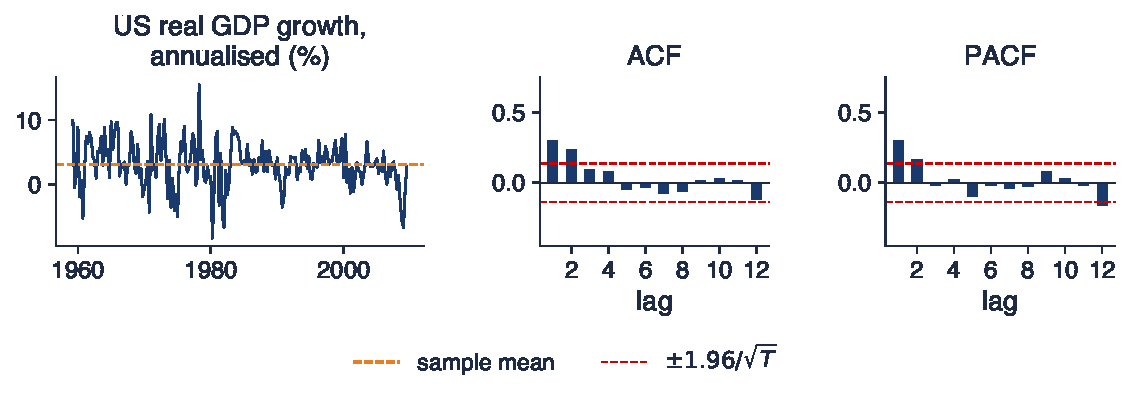
\includegraphics[width=0.96\textwidth,height=0.30\textheight,keepaspectratio]{ch2_sem_b1.pdf}
\end{center}
\vspace{-2mm}
\begin{center}
\scriptsize
\begin{tabular}{lrrrrr}
\toprule
 & WN & AR(1) & AR(2) & MA(2) & ARMA(1,1) \\
\midrule
AIC & 1084.56 & 1066.98 & \textbf{1063.70} & 1065.59 & 1065.02 \\
BIC & 1091.17 & \textbf{1076.91} & 1076.93 & 1078.83 & 1078.25 \\
\bottomrule
\end{tabular}
\end{center}
\begin{itemize}
    \item $T = 202$, ACF $0.30$, $0.24$, $0.09$ and PACF $0.30$, $0.16$, $-0.02$ (band $\pm 0.14$): AR(1) or AR(2)
    \item BIC: AR(1), $\hat\mu = 3.12$, $\hat\phi = 0.306$ (0.060); AIC: AR(2), $\hat\phi_2 = 0.163$ (0.062); the BIC values differ by 0.02
    \item AR(1) residuals: $Q^*(8) = 11.08$ on 7 df, p = 0.135; Jarque--Bera 16.0, p $<$\,0.001
    \item Interpretation: half-life $\ln 0.5/\ln 0.306 = 0.59$ quarters: growth shocks are short-lived; output levels, not growth rates, carry the persistence
\end{itemize}\quantlet{TSA\_ch2\_seminar}{\qlurl{TSA_ch2_seminar}}
\end{frame}

\begin{frame}{B2: Romanian real GDP growth [Proposed]}
\itemsize{\footnotesize}
\begin{itemize}
\item \textbf{Question}: does Romanian quarterly real GDP growth have any ARMA structure?
\item \textbf{Inputs}: Eurostat, chain-linked volumes, seasonally and calendar adjusted, 2000Q1--2026Q2; $y_t = 100\,\Delta\ln Y_t$; model: B1
\item \textbf{Tasks}
\begin{enumerate}
    \item Repeat the four steps of B1 for $y_t$ (\texttt{ro\_gdp\_growth('qoq')}).
    \item Run Ljung--Box $Q^*(8)$ on the series itself.
    \item Repeat the analysis without the four quarters of 2020, and compare.
    \item Interpretation: why is the best forecast of next quarter's growth simply the mean?
\end{enumerate}
\item \textbf{Report}: the chart, a table of ten criteria, the tests and two sentences
\item Notebook: section B2
\end{itemize}
\end{frame}

\ifsolutions
\begin{frame}{B2: solution [Proposed]}
\itemsize{\scriptsize}
\begin{center}
\includegraphics[width=0.96\textwidth,height=0.30\textheight,keepaspectratio]{ch2_sem_b2.pdf}
\end{center}
\vspace{-2mm}
\begin{center}
\scriptsize
\begin{tabular}{lrrrrr}
\toprule
 & WN & AR(1) & AR(2) & MA(2) & ARMA(1,1) \\
\midrule
AIC & \textbf{496.15} & 498.04 & 497.24 & 497.17 & 498.94 \\
BIC & \textbf{501.48} & 506.03 & 507.89 & 507.83 & 509.59 \\
\bottomrule
\end{tabular}
\end{center}
\begin{itemize}
    \item $T = 106$, mean 0.83\%, sd 2.48\%; ACF $-0.03$, $-0.16$, $-0.04$ (band $\pm 0.19$); minimum $-10.2\%$ in 2009Q1
    \item Both criteria choose white noise; $Q^*(8) = 7.5$, p = 0.481; Jarque--Bera 147.4, p $<$\,0.001; without 2020: p = 0.793, sd 2.27\%
    \item Interpretation: past quarterly growth carries no linear information about the next quarter; the forecast is $\hat\mu = 0.83\%$ (se 0.30); the annual rate of the lecture is an MA(3) because it sums four such quarters
\end{itemize}
\end{frame}
\fi

\begin{frame}{B3: BET daily returns [Solved]}
\itemsize{\footnotesize}
\begin{itemize}
\item \textbf{Question}: is the first-order autocorrelation of BET returns useful for forecasting?
\item \textbf{Inputs}: BET closes since 2000 (EODHD); $r_t = 100\,\Delta\ln P_t$, $T = 6\,670$, last day 18 September 2026
\item \textbf{Tasks}
\begin{enumerate}
    \item Estimate an AR(1) by maximum likelihood and report $\hat\phi$, its standard error and $t$-ratio, and $R^2$.
    \item Test the residuals with Ljung--Box $Q^*(10)$ on 9 degrees of freedom, and the squared residuals with $Q^*(10)$.
    \item Compute the kurtosis and the Jarque--Bera statistic of the residuals.
    \item Forecast tomorrow's return with its 95\% interval.
    \item Interpretation: is the AR(1) coefficient statistically significant, and is it economically useful?
\end{enumerate}
\item \textbf{Report}: six numbers, the chart, a forecast with its interval and two sentences
\item Notebook: section B3
\end{itemize}
\end{frame}

\begin{frame}{B3: solution [Solved]}
\itemsize{\scriptsize}
\begin{center}
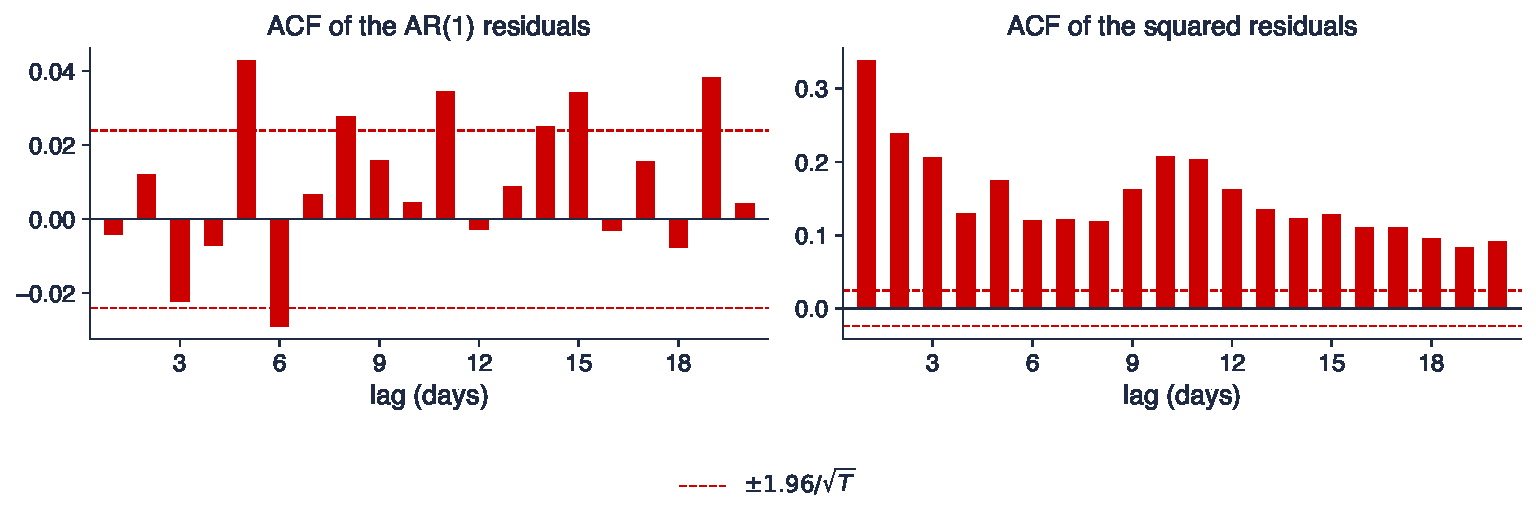
\includegraphics[width=0.96\textwidth,height=0.40\textheight,keepaspectratio]{ch2_sem_b3.pdf}
\end{center}
\vspace{-2mm}
\begin{itemize}
    \item $\hat\phi = 0.109$ (se 0.0052), $t = 20.9$; $R^2 = 1.2\%$; $\hat\sigma = 1.390\%$
    \item Residuals: $Q^*(10) = 29.7$, p $<$\,0.001 (some correlation remains); squares: $Q^*(10) = 2496$; kurtosis 14.0, Jarque--Bera 34128
    \item Last return $2.17\%$: forecast $0.294\%$, 95\% interval $[-2.43, 3.02]$ (Normal, too narrow in the tails)
    \item Interpretation: highly significant, but it explains about 1\% of the variance and the forecast is tiny relative to the interval; the large $Q^*$ of the squares points to volatility models (Chapter 5)
\end{itemize}\quantlet{TSA\_ch2\_seminar}{\qlurl{TSA_ch2_seminar}}
\end{frame}

\begin{frame}{B4: EUR/RON daily returns [Proposed]}
\itemsize{\footnotesize}
\begin{itemize}
\item \textbf{Question}: does the EUR/RON exchange rate behave like the BET?
\item \textbf{Inputs}: BNR reference rate since July 2005, $T = 5\,352$ returns; model: B3
\item \textbf{Tasks}
\begin{enumerate}
    \item Repeat the four steps of B3 (\texttt{b3\_returns('eurron')}).
    \item Compare $\hat\phi$, $R^2$ and the kurtosis with those of the BET.
    \item Interpretation: why can a managed exchange rate show a larger first-order autocorrelation than a stock index?
\end{enumerate}
\item \textbf{Report}: a table (two series, six numbers each) and two sentences
\item Notebook: section B4
\end{itemize}
\end{frame}

\ifsolutions
\begin{frame}{B4: solution [Proposed]}
\itemsize{\scriptsize}
\begin{center}
\includegraphics[width=0.96\textwidth,height=0.34\textheight,keepaspectratio]{ch2_sem_b4.pdf}
\end{center}
\vspace{-2mm}
\begin{center}
\scriptsize
\begin{tabular}{lrrrrrr}
\toprule
 & $\hat\phi$ & $t$ & $R^2$ (\%) & $Q^*(10)$ & $Q^*_{sq}(10)$ & kurtosis \\
\midrule
BET & $0.109$ & 20.9 & 1.2 & 29.7 & 2496 & 14.0 \\
EUR/RON & $0.170$ & 30.6 & 2.9 & 61.5 & 2351 & 17.0 \\
\bottomrule
\end{tabular}
\end{center}
\begin{itemize}
    \item EUR/RON: larger $\hat\phi$ and $R^2$, residual correlation left ($Q^*(10)$ p $<$\,0.001), fatter tails; forecast $0.020\%$, interval $[-0.52, 0.56]$
    \item Interpretation: the central bank smooths the rate, so moves continue for a day or two; rare large jumps give the high kurtosis
\end{itemize}
\end{frame}
\fi


%=============================================================================
\section{Part C: open questions and AI critique}
%=============================================================================

\begin{frame}{C1: does an AR model beat simple forecasts of inflation? [Proposed]}
\itemsize{\footnotesize}
\begin{itemize}
\item \textbf{Question}: is an AR(2) better than the historical mean and the last value at forecasting Romanian 12-month inflation one year ahead?
\item \textbf{Inputs}: HICP inflation since 2005 (Eurostat); forecast origins every month from January 2015; models: B1, A1
\item \textbf{Tasks}
\begin{enumerate}
    \item At each origin, estimate an AR(2) on all data up to that month and forecast 12 months ahead.
    \item Compute the same forecasts from the historical mean and from the last observed value.
    \item Compare RMSE and MAE of the three methods, over the full period and before July 2021.
    \item Interpretation: why do all three methods fail in 2022?
\end{enumerate}
\item \textbf{Report}: a table of RMSE and MAE, the chart and a plan for a project
\item Notebook: section C1
\end{itemize}
\end{frame}

\ifsolutions
\begin{frame}{C1: reference analysis [Proposed]}
\itemsize{\scriptsize}
\begin{center}
\includegraphics[width=0.96\textwidth,height=0.36\textheight,keepaspectratio]{ch2_sem_c1.pdf}
\end{center}
\vspace{-2mm}
\begin{center}
\scriptsize
\begin{tabular}{lrrr}
\toprule
 & AR(2) & mean & last value \\
\midrule
RMSE, all & 3.22 & 3.94 & 3.52 \\
MAE, all & 2.46 & 2.95 & 2.84 \\
RMSE, before July 2021 & 1.97 & 3.16 & 2.10 \\
\bottomrule
\end{tabular}
\end{center}
\begin{itemize}
    \item 128 forecasts for January 2016--August 2026; the AR(2) has the smallest errors, but its gain over the last value is small
    \item Interpretation: the 2022 energy shock was outside the history of the series; a univariate model learns it only afterwards. A project: add a formal test (Diebold--Mariano), other horizons and other countries
\end{itemize}
\end{frame}
\fi

\begin{frame}{C2: audit an AI answer [Proposed]}
\itemsize{\scriptsize}
\begin{itemize}
    \item A student asked an AI assistant about the ARMA models of this seminar. The answer:
    \item \aiprompt{(a) The process X(t) = 0.6 X(t-1) + 0.5 X(t-2) + e(t) is stationary because both coefficients are below 1.}
    \item \aiprompt{(b) An MA(1) with theta = 2 is not stationary, because |theta| > 1.}
    \item \aiprompt{(c) The AR(1) for BET returns has t = 21, so yesterday's return explains most of today's return.}
    \item \aiprompt{(d) For the residuals of an ARMA(1,1), Ljung-Box Q(8) is compared with the chi-square distribution with 8 degrees of freedom.}
    \item \aiprompt{(e) The forecast of an MA(2) three steps ahead equals the mean of the series.}
    \item \aiprompt{(f) In an AR(1), X(t) = c + phi X(t-1) + e(t), the mean of the series is c.}
    \item Tasks
    \begin{itemize}
        \item 1. For each statement, say whether it is correct; if not, give the correct statement and, where possible, the correct number from the notebook (section C2).
        \item 2. Report: a list of six verdicts with one line of justification each.
    \end{itemize}
\end{itemize}
\end{frame}

\ifsolutions
\begin{frame}{C2: solution [Proposed]}
\itemsize{\scriptsize}
\begin{itemize}
    \item (a) Wrong: $\phi_1 + \phi_2 = 1.1 > 1$; one root of $1 - 0.6z - 0.5z^2$ lies inside the circle: explosive (the lecture example C)
    \item (b) Wrong: every finite MA is stationary; $|\theta| > 1$ breaks invertibility, not stationarity (A3)
    \item (c) Wrong: significant is not large: $\hat\phi = 0.109$, $\hat\phi^2 \approx 1.2\%$ of the variance (B3)
    \item (d) Wrong: $8 - p - q = 6$ degrees of freedom; with 8 the test is too lenient (A6)
    \item (e) Correct: beyond $q = 2$ steps the forecast is $\mu$
    \item (f) Wrong: the mean is $c/(1 - \phi)$; $c$ is the intercept (A1)
\end{itemize}\quantlet{TSA\_ch2\_seminar}{\qlurl{TSA_ch2_seminar}}
\end{frame}
\fi


%=============================================================================
\section{Wrap-up}
%=============================================================================

\begin{frame}{Key takeaways}
\itemsize{\small}
\begin{itemize}
    \item Stationarity is read from the roots of $\phi(z)$, invertibility from the roots of $\theta(z)$, never from single coefficients
    \item The mean of an AR model is $c/\phi(1)$, not the intercept $c$
    \item Box--Jenkins: ACF and PACF propose, AIC and BIC choose, residual tests check, forecasts are compared with simple benchmarks
    \item Ljung--Box on residuals uses $m - p - q$ degrees of freedom
    \item Statistically significant is not economically large: compare $\hat\phi^2$ with the forecast interval
\end{itemize}
\end{frame}

\begin{frame}{After the seminar}
\itemsize{\small}
\begin{itemize}
    \item Lecture 2 derives today's formulas: roots, invertibility, $\psi$ weights, estimators, information criteria, forecast intervals, the Box--Jenkins case of Romanian GDP
    \item Try the [Proposed] tasks in the notebook
    \item C1 can grow into a team project: ARMA forecasts of inflation in Romania and the region against simple benchmarks
    \item Reading: \refHP, Ch.~3--4; \refFPP, Ch.~9; \refBD, Ch.~3
    \item \textbf{The seminar is for practice and is not graded; the solutions of [Proposed] tasks are discussed in class}
\end{itemize}
\end{frame}


%=============================================================================
\section{References}
%=============================================================================

\begin{frame}{References}
\itemsize{\tiny}
\begin{itemize}
    \item Akaike, H. (1974). A new look at the statistical model identification. \textit{IEEE Transactions on Automatic Control}, 19(6), 716--723. \href{https://doi.org/10.1109/TAC.1974.1100705}{doi:10.1109/TAC.1974.1100705}
    \item Box, G. E. P., Jenkins, G. M., \& Reinsel, G. C. (2008). \textit{Time Series Analysis: Forecasting and Control} (4th ed.). Wiley. \href{https://doi.org/10.1002/9781118619193}{doi:10.1002/9781118619193}
    \item Box, G. E. P., \& Pierce, D. A. (1970). Distribution of residual autocorrelations in autoregressive-integrated moving average time series models. \textit{Journal of the American Statistical Association}, 65(332), 1509--1526. \href{https://doi.org/10.1080/01621459.1970.10481180}{doi:10.1080/01621459.1970.10481180}
    \item Brockwell, P. J., \& Davis, R. A. (2016). \textit{Introduction to Time Series and Forecasting} (3rd ed.). Springer. \href{https://doi.org/10.1007/978-3-319-29854-2}{doi:10.1007/978-3-319-29854-2}
    \item Huang, C., \& Petukhina, A. (2022). \textit{Applied Time Series Analysis and Forecasting with Python}. Springer. \href{https://doi.org/10.1007/978-3-031-13584-2}{doi:10.1007/978-3-031-13584-2}
    \item Hyndman, R. J., \& Athanasopoulos, G. (2021). \textit{Forecasting: Principles and Practice} (3rd ed.). OTexts. \href{https://otexts.com/fpp3/}{otexts.com/fpp3}
    \item Jarque, C. M., \& Bera, A. K. (1987). A test for normality of observations and regression residuals. \textit{International Statistical Review}, 55(2), 163--172. \href{https://doi.org/10.2307/1403192}{doi:10.2307/1403192}
    \item Ljung, G. M., \& Box, G. E. P. (1978). On a measure of lack of fit in time series models. \textit{Biometrika}, 65(2), 297--303. \href{https://doi.org/10.1093/biomet/65.2.297}{doi:10.1093/biomet/65.2.297}
    \item Schwarz, G. (1978). Estimating the dimension of a model. \textit{The Annals of Statistics}, 6(2), 461--464. \href{https://doi.org/10.1214/aos/1176344136}{doi:10.1214/aos/1176344136}
\end{itemize}
\end{frame}

\end{document}
